%\documentclass[a4paper,twocolumn]{article} % Document type

\documentclass[a4paper,12pt,oneside,onecolumn]{article} % Document type

\usepackage[left=1.0in, right=1.0in, top=1.0in, bottom=1.0in]{geometry}
\usepackage{float}
\usepackage{subcaption}
\usepackage{tikz}
\usetikzlibrary{automata,positioning}
	
\usepackage{mathrsfs}

\ifx\pdfoutput\undefined
    %Use old Latex if PDFLatex does not work
  \usepackage[dvips]{graphicx}% To get graphics working
 \DeclareGraphicsExtensions{.eps} % Encapsulated PostScript
 \else
    %Use PDFLatex
   \usepackage[pdftex]{graphicx}% To get graphics working
   \DeclareGraphicsExtensions{.pdf,.jpg,.png,.mps,} % Portable Document Format, Joint Photographic Experts Group, Portable Network Graphics, MetaPost
   \pdfcompresslevel=9
\fi

\usepackage{amsmath,amssymb}   % Contains mathematical symbols

\usepackage[ansinew]{inputenc} % Input encoding, identical to Windows 1252
\usepackage[english]{babel}    % Language
\usepackage[square,numbers]{natbib}     %Nice numbered citations
\bibliographystyle{plainnat}            %Sorted bibliography



\begin{document}               % Begins the document

\title{Homework 3 (Tasks 1-19) in EL2450 Hybrid and Embedded Control Systems}
\author{
  Sindhuja Balaji \\ 930831-0748 \\ sindhuja@kth.se
  \and
  Tobias Bolin \\ 870702-0098 \\ tbolin@kth.se
  \and
  Yue Jiao \\ 911024-7799 \\ yj@kth.se
  \and
 Ida Karlsson \\ 930705-6102 \\ ikarlss@kth.se
  \and
  }
%\date{2010-10-10}             % If you want to set the date yourself.

\maketitle                     % Generates the title




%%%%%%%%%%%%%%%%%%%%%%%%%%%%%%%%%%%%%%%%%%%%%%%%%%%%%%%%%%%%%%%%%%%%%%%%%%%%%%%%%%%
% Instructions regarding the report
%%%%%%%%%%%%%%%%%%%%%%%%%%%%%%%%%%%%%%%%%%%%%%%%%%%%%%%%%%%%%%%%%%%%%%%%%%%%%%%%%%%



\section*{Task 1}

Given:
 \begin{align*}
  v&=\frac{u_r+u_l}{2}\\
 \omega&=u_r-u_l \rightarrow\\
 &2v+\omega=2u_r\\
 &2v-\omega=2u_l\rightarrow \\
 u_r&=v+\frac{1}{2}\omega\\
 u_l&=v-\frac{1}{2}\omega
 \end{align*}
 

\section*{Task 2}

The field was discretized in equally sized squares of $50 \times 50 cm$ for a total of $K=36$ states.  
 
 \begin{figure}[H]
 \centering
  \includegraphics[width = 0.8\textwidth]{hw3_map.png}
  \caption{The discretized field}
  \end{figure}

The regions are defined as: $R_i$ for $i\in \{1,..,36\}$


 The transition system is a tuple in the form:
$\mathcal{T}=(S,S_0,\sum,\rightarrow,\Pi,\mathcal{L})$\\
The defined states $S=\{R_1,R_2,...R_{36}\}.$\\
$\Pi=\{R,G,B,O\}$\\
The corresponding labels:\\
$\mathcal{L}(R_1)=\{R\}$\\
$\mathcal{L}(R_2)=\{G\}$\\
$\mathcal{L}(R_3)=\{O\}$\\
$\mathcal{L}(R_4)=\{\}$\\
$\mathcal{L}(R_5)=\{\}$\\
$\mathcal{L}(R_6)=\{G\}$\\
$\mathcal{L}(R_7)=\{B\}$\\
$\mathcal{L}(R_8)=\{R,O\}$\\
$\mathcal{L}(R_9)=\{G\}$\\
$\mathcal{L}(R_{10})=\{O\}$\\
$\mathcal{L}(R_{11})=\{R,O\}$\\
$\mathcal{L}(R_{12})=\{\}$\\
$\mathcal{L}(R_{13})=\{\}$\\
$\mathcal{L}(R_{14})=\{\}$\\
$\mathcal{L}(R_{15})=\{\}$\\
$\mathcal{L}(R_{16})=\{\}$\\
$\mathcal{L}(R_{17})=\{\}$\\
$\mathcal{L}(R_{18})=\{\}$\\
$\mathcal{L}(R_{19})=\{O\}$\\
$\mathcal{L}(R_{20})=\{R\}$\\
$\mathcal{L}(R_{21})=\{B\}$\\
$\mathcal{L}(R_{22})=\{O\}$\\
$\mathcal{L}(R_{23})=\{B\}$\\
$\mathcal{L}(R_{24})=\{\}$\\
$\mathcal{L}(R_{25})=\{\}$\\
$\mathcal{L}(R_{26})=\{B,O\}$\\
$\mathcal{L}(R_{27})=\{\}$\\
$\mathcal{L}(R_{28})=\{\}$\\
$\mathcal{L}(R_{29})=\{R,O\}$\\
$\mathcal{L}(R_{30})=\{G\}$\\
$\mathcal{L}(R_{31})=\{R,G\}$\\
$\mathcal{L}(R_{32})=\{R\}$\\
$\mathcal{L}(R_{33})=\{\}$\\
$\mathcal{L}(R_{34})=\{\}$\\
$\mathcal{L}(R_{35})=\{\}$\\
$\mathcal{L}(R_{36})=\{B\}$\\

The actions:
$\sum=\{N,S,W,E\}$.\\
The transitions can be seen in figure \ref{fig:INT}. 
%a_N-North (up), a_S=south (down), a_W-west (left), a_E-east (right)
%adds transition image
\begin{figure}[H]
    \centering

    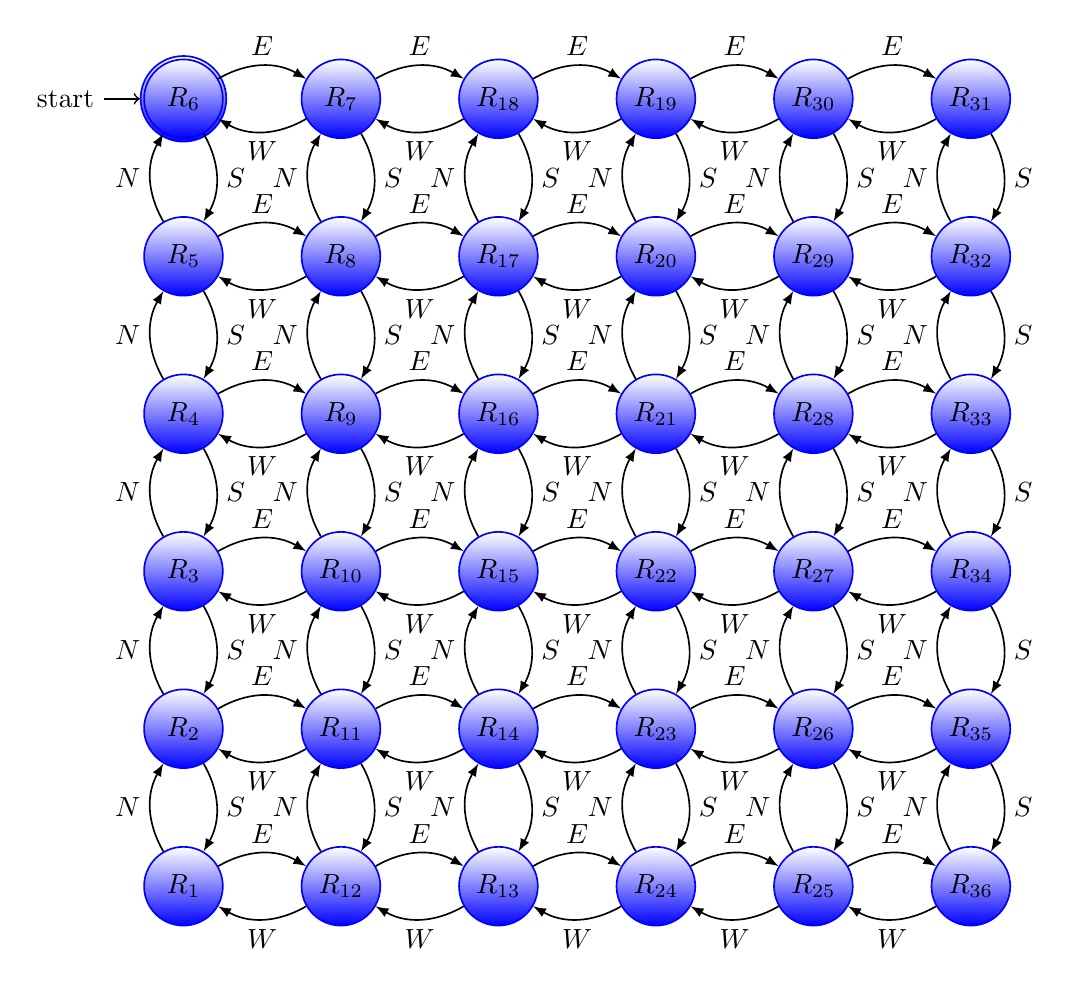
\begin{tikzpicture}[-latex ,auto ,node distance =2 cm and 2cm  ,semithick ,state/.style ={ circle ,top color =white , bottom color =blue ,draw,blue , text=black , minimum width =1 cm}]
    \node[state,initial ,initial where=left,] (R_6)   {$q_\text{start}$};
    
    \node[state] (R_6) {$R_6$};
    \node[state] (R_5) [below of=R_6] {$R_5$};
    \node[state] (R_4) [below of=R_5] {$R_4$};
    \node[state] (R_3) [below of=R_4] {$R_3$};
    \node[state] (R_2) [below of=R_3] {$R_2$};
    \node[state] (R_1) [below of=R_2] {$R_1$};
    
    \node[state] (R_7) [right of=R_6] {$R_7$};
    \node[state] (R_8) [below of=R_7] {$R_8$};
    \node[state] (R_9) [below of=R_8] {$R_9$};
    \node[state] (R_10) [below of=R_9] {$R_{10}$};
    \node[state] (R_11) [below of=R_10] {$R_{11}$};
    \node[state] (R_12) [below of=R_11] {$R_{12}$};

    \node[state] (R_18) [right of=R_7] {$R_{18}$};
    \node[state] (R_17) [below of=R_18] {$R_{17}$};
    \node[state] (R_16) [below of=R_17] {$R_{16}$};
    \node[state] (R_15) [below of=R_16] {$R_{15}$};
    \node[state] (R_14) [below of=R_15] {$R_{14}$};
    \node[state] (R_13) [below of=R_14] {$R_{13}$};
    
    \node[state] (R_19) [right of=R_18] {$R_{19}$};
    \node[state] (R_20) [below of=R_19] {$R_{20}$};
    \node[state] (R_21) [below of=R_20] {$R_{21}$};
    \node[state] (R_22) [below of=R_21] {$R_{22}$};
    \node[state] (R_23) [below of=R_22] {$R_{23}$};
    \node[state] (R_24) [below of=R_23] {$R_{24}$};

    \node[state] (R_30) [right of=R_19] {$R_{30}$};
    \node[state] (R_29) [below of=R_30] {$R_{29}$};
    \node[state] (R_28) [below of=R_29] {$R_{28}$};
    \node[state] (R_27) [below of=R_28] {$R_{27}$};
    \node[state] (R_26) [below of=R_27] {$R_{26}$};
    \node[state] (R_25) [below of=R_26] {$R_{25}$};
    
    \node[state] (R_31) [right of=R_30] {$R_{31}$};
    \node[state] (R_32) [below of=R_31] {$R_{32}$};
    \node[state] (R_33) [below of=R_32] {$R_{33}$};
    \node[state] (R_34) [below of=R_33] {$R_{34}$};
    \node[state] (R_35) [below of=R_34] {$R_{35}$};
    \node[state] (R_36) [below of=R_35] {$R_{36}$};
%paths
    \path (R_1) edge [bend left] node {$N$} (R_2);
    \path (R_1) edge [bend left] node {$E$} (R_12);
    
    \path (R_2) edge [bend left] node {$N$} (R_3);
    \path (R_2) edge [bend left] node {$E$} (R_11);
    \path (R_2) edge [bend left] node {$S$} (R_1);
    
    \path (R_3) edge [bend left] node {$N$} (R_4);
    \path (R_3) edge [bend left] node {$E$} (R_10);
    \path (R_3) edge [bend left] node {$S$} (R_2);

    
    \path (R_4) edge [bend left] node {$N$} (R_5);
    \path (R_4) edge [bend left] node {$E$} (R_9);
    \path (R_4) edge [bend left] node {$S$} (R_3);
    
    \path (R_5) edge [bend left] node {$N$} (R_6);
    \path (R_5) edge [bend left] node {$E$} (R_8);
    \path (R_5) edge [bend left] node {$S$} (R_4);
    
    \path (R_6) edge [bend left] node {$E$} (R_7);
    \path (R_6) edge [bend left] node {$S$} (R_5);
    
    \path (R_7) edge [bend left] node {$S$} (R_8);
    \path (R_7) edge [bend left] node {$E$} (R_18);
    \path (R_7) edge [bend left] node {$W$} (R_6);
    
    \path (R_8) edge [bend left] node {$N$} (R_7);
    \path (R_8) edge [bend left] node {$S$} (R_9);
    \path (R_8) edge [bend left] node {$E$} (R_17);
    \path (R_8) edge [bend left] node {$W$} (R_5);
    
    \path (R_9) edge [bend left] node {$N$} (R_8);
    \path (R_9) edge [bend left] node {$S$} (R_10);
    \path (R_9) edge [bend left] node {$E$} (R_16);
    \path (R_9) edge [bend left] node {$W$} (R_4);
    
    \path (R_10) edge [bend left] node {$N$} (R_9);
    \path (R_10) edge [bend left] node {$S$} (R_11);
    \path (R_10) edge [bend left] node {$E$} (R_15);
    \path (R_10) edge [bend left] node {$W$} (R_3);
    
    \path (R_11) edge [bend left] node {$N$} (R_10);
    \path (R_11) edge [bend left] node {$S$} (R_12);
    \path (R_11) edge [bend left] node {$E$} (R_14);
    \path (R_11) edge [bend left] node {$W$} (R_2);
    
    \path (R_12) edge [bend left] node {$N$} (R_11);
    \path (R_12) edge [bend left] node {$E$} (R_13);
    \path (R_12) edge [bend left] node {$W$} (R_1);
    
    \path (R_13) edge [bend left] node {$N$} (R_14);
    \path (R_13) edge [bend left] node {$W$} (R_12);
    \path (R_13) edge [bend left] node {$E$} (R_24);
    
    \path (R_14) edge [bend left] node {$S$} (R_13);
    \path (R_14) edge [bend left] node {$N$} (R_15);
    \path (R_14) edge [bend left] node {$W$} (R_11);
    \path (R_14) edge [bend left] node {$E$} (R_23);
    
    \path (R_15) edge [bend left] node {$N$} (R_16);
    \path (R_15) edge [bend left] node {$S$} (R_14);
    \path (R_15) edge [bend left] node {$E$} (R_22);
    \path (R_15) edge [bend left] node {$W$} (R_10);
    
\path (R_16) edge [bend left] node {$N$} (R_17);
    \path (R_16) edge [bend left] node {$S$} (R_15);
    \path (R_16) edge [bend left] node {$E$} (R_21);
    \path (R_16) edge [bend left] node {$W$} (R_9);
    
    \path (R_17) edge [bend left] node {$N$} (R_18);
    \path (R_17) edge [bend left] node {$S$} (R_16);
    \path (R_17) edge [bend left] node {$E$} (R_20);
    \path (R_17) edge [bend left] node {$W$} (R_8);
    
    \path (R_18) edge [bend left] node {$E$} (R_19);
    \path (R_18) edge [bend left] node {$S$} (R_17);
    \path (R_18) edge [bend left] node {$W$} (R_7);
    
    \path (R_19) edge [bend left] node {$S$} (R_20);
    \path (R_19) edge [bend left] node {$W$} (R_18);
    \path (R_19) edge [bend left] node {$E$} (R_30);
    
    \path (R_20) edge [bend left] node {$S$} (R_21);
    \path (R_20) edge [bend left] node {$N$} (R_19);
    \path (R_20) edge [bend left] node {$E$} (R_29);
    \path (R_20) edge [bend left] node {$W$} (R_17);
    
    \path (R_21) edge [bend left] node {$S$} (R_22);
    \path (R_21) edge [bend left] node {$N$} (R_20);
    \path (R_21) edge [bend left] node {$E$} (R_28);
    \path (R_21) edge [bend left] node {$W$} (R_16);
    
    \path (R_22) edge [bend left] node {$S$} (R_23);
    \path (R_22) edge [bend left] node {$N$} (R_21);
    \path (R_22) edge [bend left] node {$E$} (R_27);
    \path (R_22) edge [bend left] node {$W$} (R_15);
    
    \path (R_23) edge [bend left] node {$S$} (R_24);
    \path (R_23) edge [bend left] node {$N$} (R_22);
    \path (R_23) edge [bend left] node {$E$} (R_26);
    \path (R_23) edge [bend left] node {$W$} (R_14);
        
    \path (R_24) edge [bend left] node {$E$} (R_25);
    \path (R_24) edge [bend left] node {$N$} (R_23);
    \path (R_24) edge [bend left] node {$W$} (R_13);
    
    \path (R_25) edge [bend left] node {$N$} (R_26);
    \path (R_25) edge [bend left] node {$W$} (R_24);
    \path (R_25) edge [bend left] node {$E$} (R_36);
    
    \path (R_26) edge [bend left] node {$S$} (R_25);
    \path (R_26) edge [bend left] node {$N$} (R_27);
    \path (R_26) edge [bend left] node {$W$} (R_23);
    \path (R_26) edge [bend left] node {$E$} (R_35);
    
    \path (R_27) edge [bend left] node {$N$} (R_28);
    \path (R_27) edge [bend left] node {$S$} (R_26);
    \path (R_27) edge [bend left] node {$E$} (R_34);
    \path (R_27) edge [bend left] node {$W$} (R_22);
    
    \path (R_28) edge [bend left] node {$N$} (R_29);
    \path (R_28) edge [bend left] node {$S$} (R_27);
    \path (R_28) edge [bend left] node {$W$} (R_21);
    \path (R_28) edge [bend left] node {$E$} (R_33);
    
    \path (R_29) edge [bend left] node {$N$} (R_30);
    \path (R_29) edge [bend left] node {$S$} (R_28);
    \path (R_29) edge [bend left] node {$E$} (R_32);
    \path (R_29) edge [bend left] node {$W$} (R_20);
    
    \path (R_30) edge [bend left] node {$E$} (R_31);
    \path (R_30) edge [bend left] node {$S$} (R_29);
    \path (R_30) edge [bend left] node {$W$} (R_19);
    
    \path (R_31) edge [bend left] node {$S$} (R_32);
    \path (R_31) edge [bend left] node {$W$} (R_30);
    
    \path (R_32) edge [bend left] node {$S$} (R_33);
    \path (R_32) edge [bend left] node {$N$} (R_31);
    \path (R_32) edge [bend left] node {$W$} (R_29);
    
    
    \path (R_33) edge [bend left] node {$N$} (R_32);
    \path (R_33) edge [bend left] node {$S$} (R_34);
    \path (R_33) edge [bend left] node {$W$} (R_28);
    
    
    \path (R_34) edge [bend left] node {$N$} (R_33);
    \path (R_34) edge [bend left] node {$S$} (R_35);
    \path (R_34) edge [bend left] node {$W$} (R_27);
    
    
    \path (R_35) edge [bend left] node {$S$} (R_36);
    \path (R_35) edge [bend left] node {$N$} (R_34);
    \path (R_35) edge [bend left] node {$W$} (R_26);
    
    
    \path (R_36) edge [bend left] node {$N$} (R_35);
    \path (R_36) edge [bend left] node {$W$} (R_25);
    
    \end{tikzpicture}
    \caption{The transition system.}
    \label{fig:INT}
\end{figure}


\section*{Task 3}

If the robot uses the path $p=R_{13},R_{14},R_{15},R_{16},R_{17},R_{20},R_{21},R_{28},R_{33},R_{34},R_{35},R_{36},R_{25},R_{R_24},R_{13}...$ it will go in an infinite loop passing a red state infinite times. Never passing an obstacle and after each time it passes a red state it passes a blue state right after. Se figure \ref{inf_path}
\begin{figure}[H]
 \centering
  \includegraphics[width = 0.8\textwidth]{hw3_map_path.png}
  \caption{The infinite path}
  \label{inf_path}
  \end{figure}


\section*{Task 4}

If both the distance and relative orientation of the robot are controlled at the same time, the robot might start driving in a direction that takes it into another region than the goal region. Making sure that the robot is aligned towards the correct region before any translational motion ensures that the robot will stay in a valid state. Beside this situation, the movement might take long time if the desired orientation differs greatly from the desired movement direction. This is because that the robot tries to maintain in the direction that is not the movement direction so it will constantly stop and rotate toward the desired direction and rotate back to continue moving without any benefit. So it is better to move to the desired location before rotate to the desired direction. 

\section*{Task 5}

In order for a discrete time system to be stable the eigenvalues of the system must have a magnitude less then 1. 

From the dynamics of the system we have that
\begin{align*}
%    \omega[k]&=K_\psi(\theta^R-\theta[k])\\
%    &\Rightarrow\\
    \theta[k+1]&=\theta[k]+ \frac{R}{L} K_\psi(\theta^R-\theta[k])\\
    \theta[k+1]&=(1- \frac{R}{L} K_\psi)\theta[k]+K_\psi\theta^R
\end{align*} The system's eigenvalue, $\lambda$ is given by $1 - \frac{R}{L} K_\psi$ and the system is asymptotically stable if $|\lambda| > 1.$ 
If $1 - \frac{R}{L} K_\psi = 0$ the right hand side of the system is equal to $\theta^R$ and we have a deadbeat controller. So we chose
\[
K_\omega = \frac{L}{R} \approx 5.05.
\]


\section*{Task 6}


\begin{equation}
\begin{aligned}
    \omega = u_r - u_l = K_\psi (\theta^R-\theta)& , \quad v = \frac{u_r + u_l}{2}= 0 \\
    u_r = \frac{K\psi(\theta^R - \theta)}{2}&, \quad u_l = - u_r
\end{aligned}
\end{equation}

Simulation results using $K_\psi=5$.

\begin{figure}[H]
    \centering
    \begin{subfigure}[b]{7cm}
        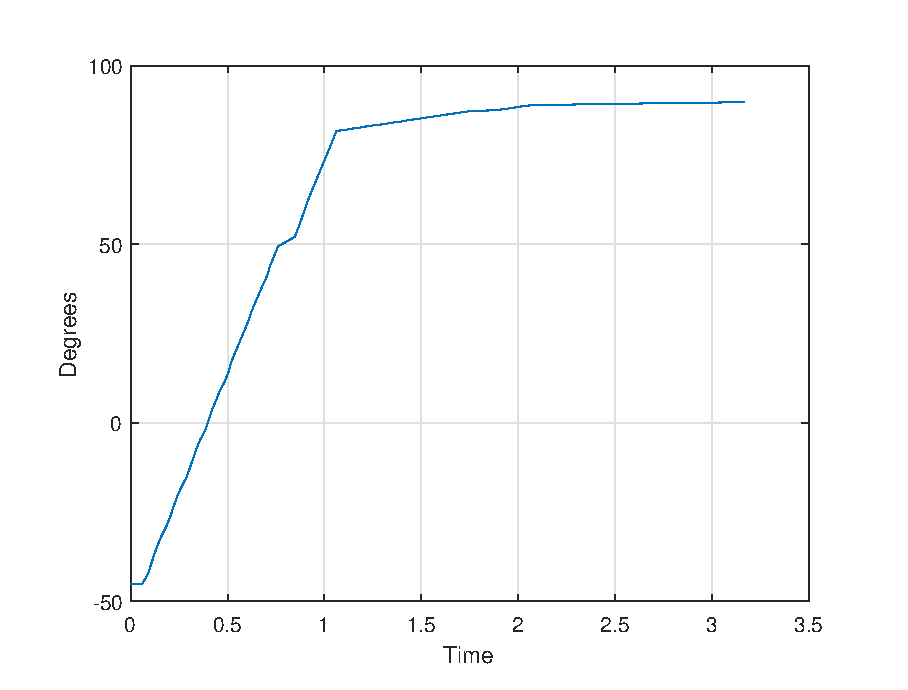
\includegraphics[width=\textwidth]{rotation_m45.eps}
        \caption{Initial angle: -45 degrees}
        \label{fig:m45deg}
    \end{subfigure}
    \begin{subfigure}[b]{7cm}
        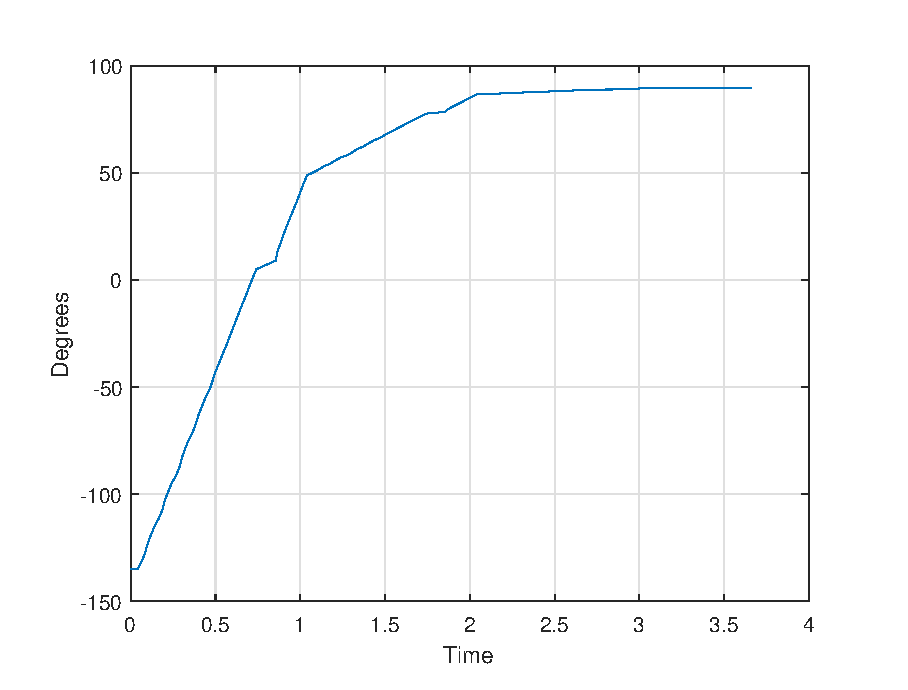
\includegraphics[width=\textwidth]{rotation_m135.eps}
        \caption{Initial angle: -135 degrees}
        \label{fig:m135deg}
    \end{subfigure}
   
   
    \begin{subfigure}[b]{7cm}
        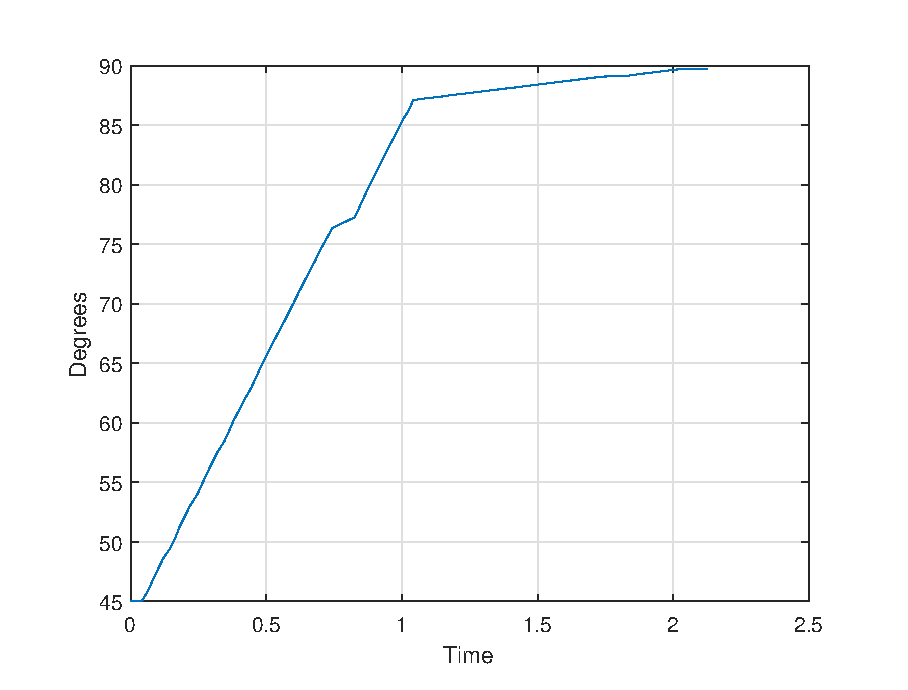
\includegraphics[width=\textwidth]{rotation_p45.eps}
        \caption{Initial angle: 45 degrees}
        \label{fig:45deg}
    \end{subfigure}
     \begin{subfigure}[b]{7cm}
        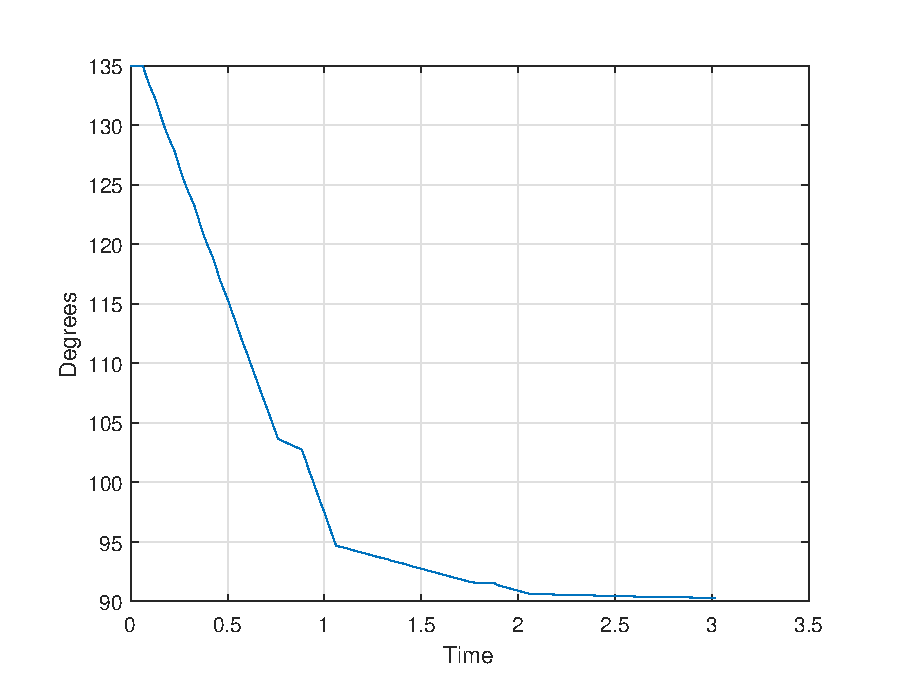
\includegraphics[width=\textwidth]{rotation_p135.eps}
        \caption{Initial angle: 135 degrees}
        \label{fig:135deg}
    \end{subfigure}
    \caption{Rotation, $K_\psi=5$, $\theta^R=90$ degrees}\label{fig:animals}
    \label{fig:dir-ctrl}
\end{figure}

As shown in task 5 it should be possible to maintain $\theta[k]$ at $\theta^R.$ However this does not account for the quantization error, which exists in both the measurements and the output, which might introduce a small offset. Task 5 does not account for any constant disturbances either, which would require an I controller to fix. It also assumes that the output will be constant during the time between samples. In all the plots in Fig \ref{fig:dir-ctrl} a small decrease in angular velocity can be seen at around $0.75$ seconds after each sample. This will slow down the controller and might make $\theta[k]$ go towards $\theta^R$ asymptotically, but not reaching it in finite time. 
%\begin{equation}
%\begin{aligned}
%    \omega = \dot{\theta} = K_\psi(\theta^R-\theta)  \Rightarrow \\
%    \dot{\theta} + K_\psi \theta - K_\psi \theta_\psi = 0 \Rightarrow \\
%    \theta = \theta^R + C e^{-K_\psi t}  \Rightarrow \\
%    \theta \rightarrow \theta^R \textrm{ as } t \rightarrow \infty
%\end{aligned}
%\end{equation}
%So it is possible to maintain $\theta=\theta^R$. 

\section*{Task 7}


Per definition
\[
d_0[k+1] = \Delta_0[k+1] \cdot v_c[k+1].
\]
Then, with the position $p[k]$, $\Delta_0[k+1] = \Delta_0[k] + p[k] - p[k+1].$ 
The position in the next time step is given by $p[k+1] = p[k] + R\frac{\pi}{180}v[k] v_c[k].$ The $R\frac{\pi}{180}$ coefficient is necessary to change the unit of $v$ from degrees per second into meters per second. Substituting in the controller into this equation gives $p[k+1] = p[k] + KR\frac{\pi}{180}d_0[k] v_c[k].$
Inserting this expression into the equation for $\Delta_0[k+1]$ we get $\Delta_0[k+1] = \Delta_0[k] - K_\omega R\frac{\pi}{180}d_0[k] v_c[k].$

If we assume that $\theta$ is constant, then $v_c[k+1] = v_c[k],$
so $d_0 [k+1] = (\Delta_0[k] - R\frac{\pi}{180}d_0[k] v_c[k])\cdot v_c[k].$ Since $\Delta_0[k] \cdot v_c[k] = d_0[k]$ and $v_c[k]\cdot v_c[k] = 1$ we finally get
\begin{equation*}
d_0 [k+1] = (1-K_\omega \frac{\pi}{180})d_0[k].
\end{equation*}

The eigenvalue of this system is given by $1-K_\omega \frac{\pi}{180}.$ If $K_\omega > 2\frac{180}{R \pi}$ the system will become unstable. $K_\omega = \frac{180}{R \pi} \approx 572$ gives a dead beat controller.


\section*{Task 8}

Simulations results using $K_\omega=500$:

% d0 Controller
\begin{figure}[H]
    \centering
    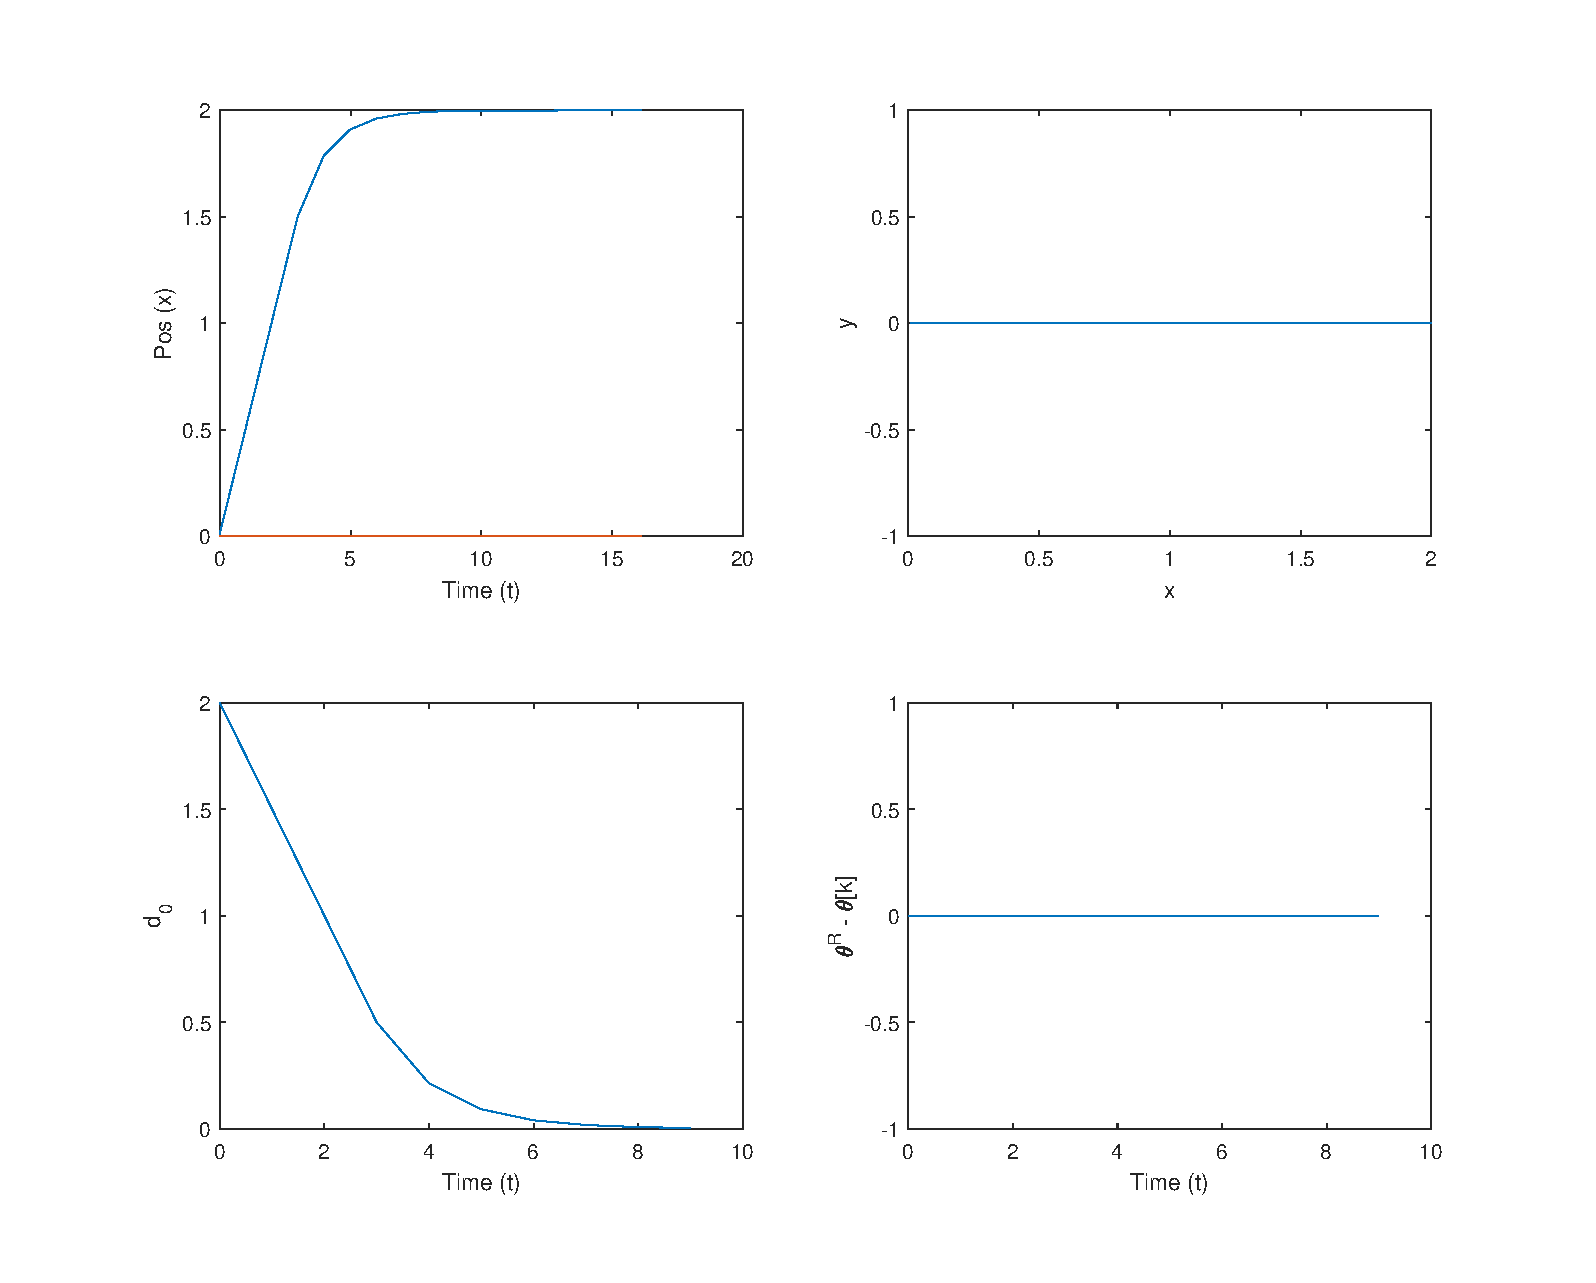
\includegraphics[width=\textwidth]{figs/perf-d0.eps}
    %\begin{subfigure}[b]{7cm}
    %    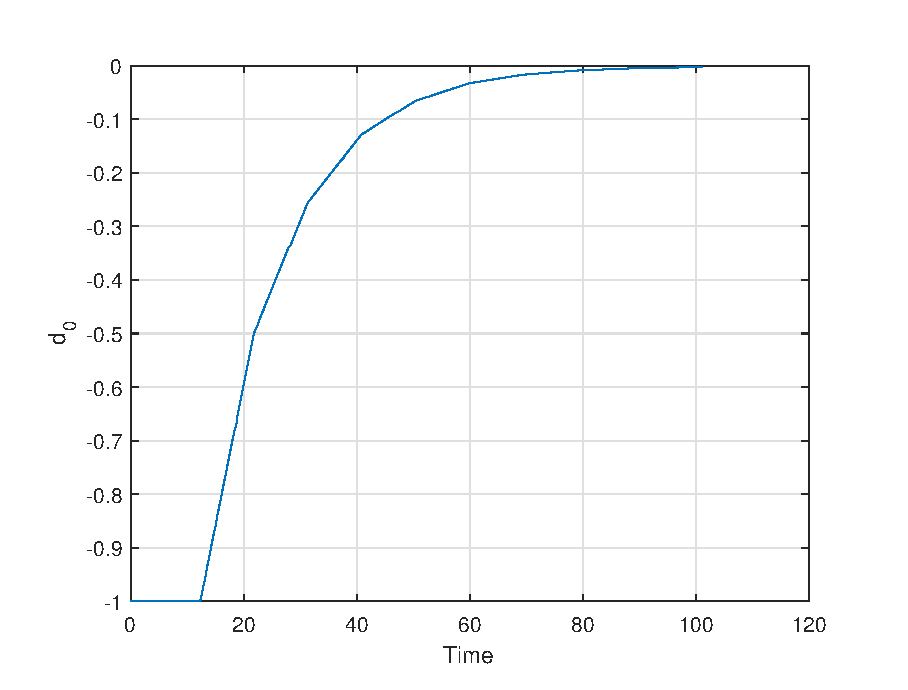
\includegraphics[width=\textwidth]{task8_500_d0_initial_00_Goal_11.eps}
    %    \caption{Initial position: (0,0), Goal: (1,1)}
    %    \label{fig:500d00011}
    %\end{subfigure}
    %\begin{subfigure}[b]{7cm}
    %    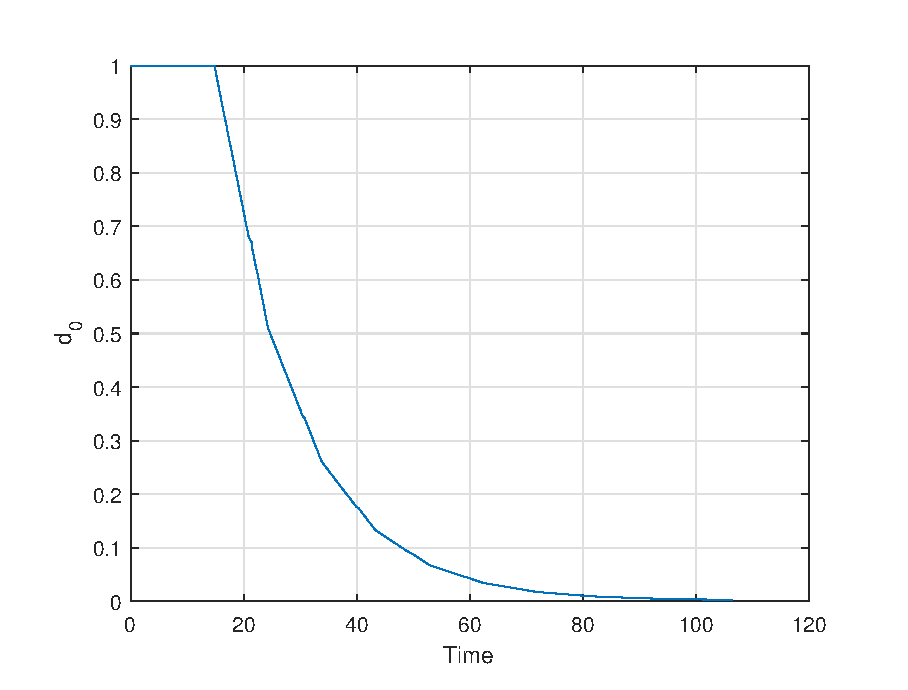
\includegraphics[width=\textwidth]{task8_500_d0_initial_21_Goal_11.eps}
    %    \caption{Initial position: (2,1), Goal: (1,1) }
    %    \label{fig:d05002111}
    %\end{subfigure}
    %
    %
    %\begin{subfigure}[b]{7cm}
    %    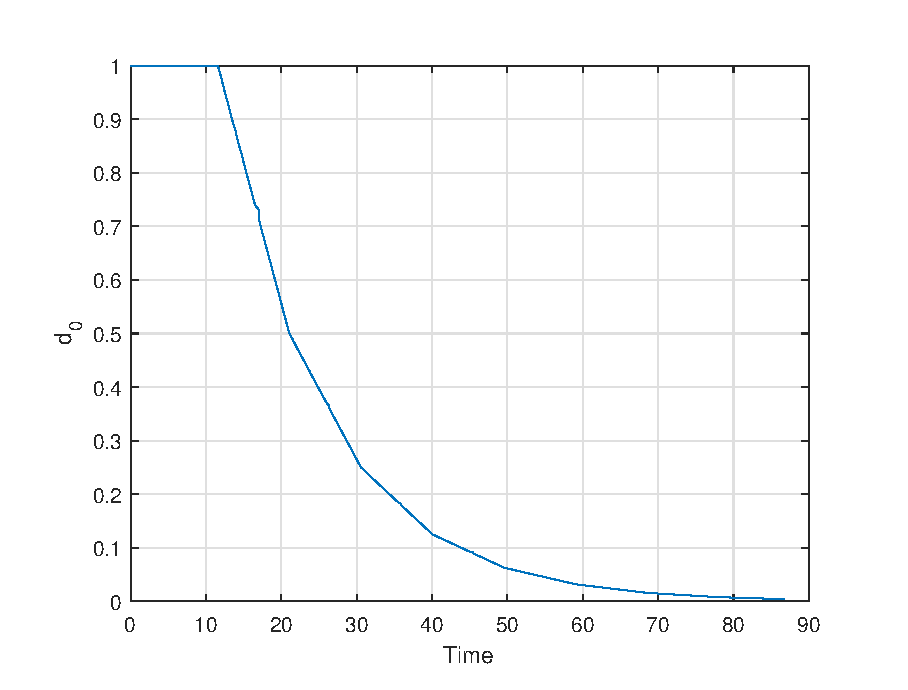
\includegraphics[width=\textwidth]{task8_500_d0_initial_11_Goal_02.eps}
    %    \caption{Initial position: (1,1), Goal: (0,2)}
    %    \label{fig:d05001102}
    %\end{subfigure}
    % \begin{subfigure}[b]{7cm}
    %    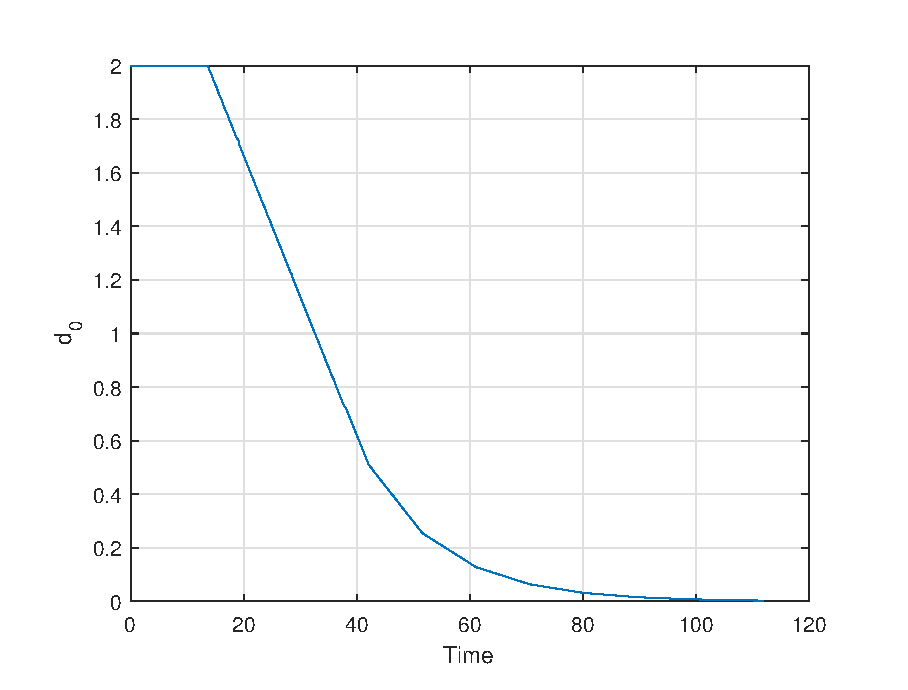
\includegraphics[width=\textwidth]{task8_500_d0_initial_20_Goal_02.eps}
    %    \caption{Initial position: (2,0), Goal: (0,2) }
    %    \label{fig:d05002002}
    %\end{subfigure}
    
    \caption{Simulation of the $d_0$ controller going from $(0, 0)$ to $(2, 2)$ with $K_\omega= \frac{180}{R \pi}.$}\label{fig:d02002}
\end{figure}

The controller drives the robot to a position orthogonal to the goal position where the value $d_0$ is zero. If the robot is aligned with the line from the initial position to the goal, then the robot will reach the goal position. Otherwise it will not.\textbf{}

\section*{Task 9}

Simulation results when using both controllers with $K_\omega=500$ and $K_\psi=5$. 
\begin{figure}[H]
    \centering
    
    \begin{subfigure}[b]{6cm}
        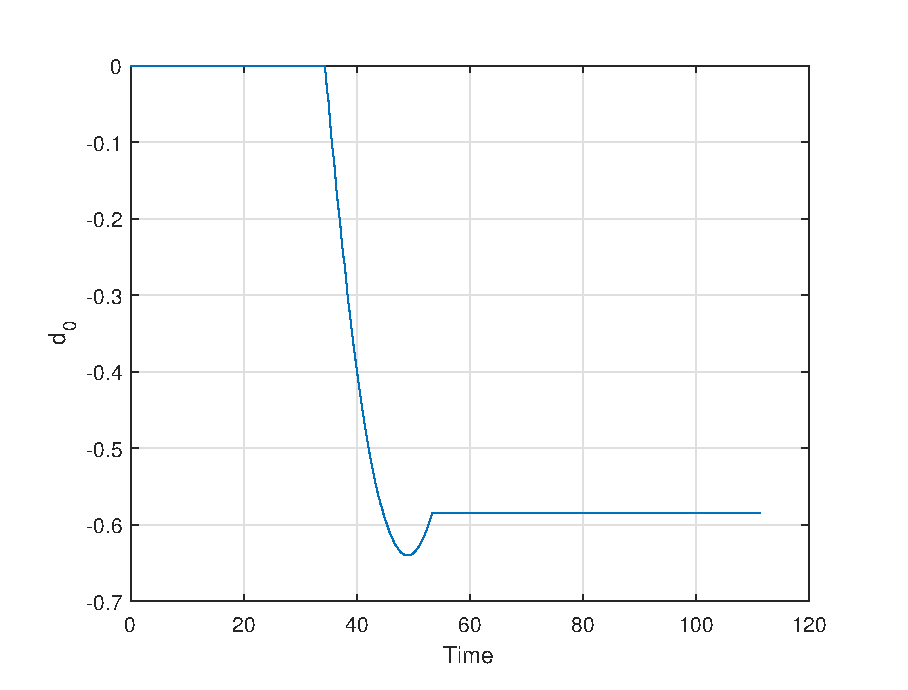
\includegraphics[width=\textwidth]{task_9_500_d0_initial_000_Goal_2090.eps}
        \caption{Initial position: (0,0) 0 degrees}
        \label{fig:d0002090}
    \end{subfigure}
    \begin{subfigure}[b]{6cm}
        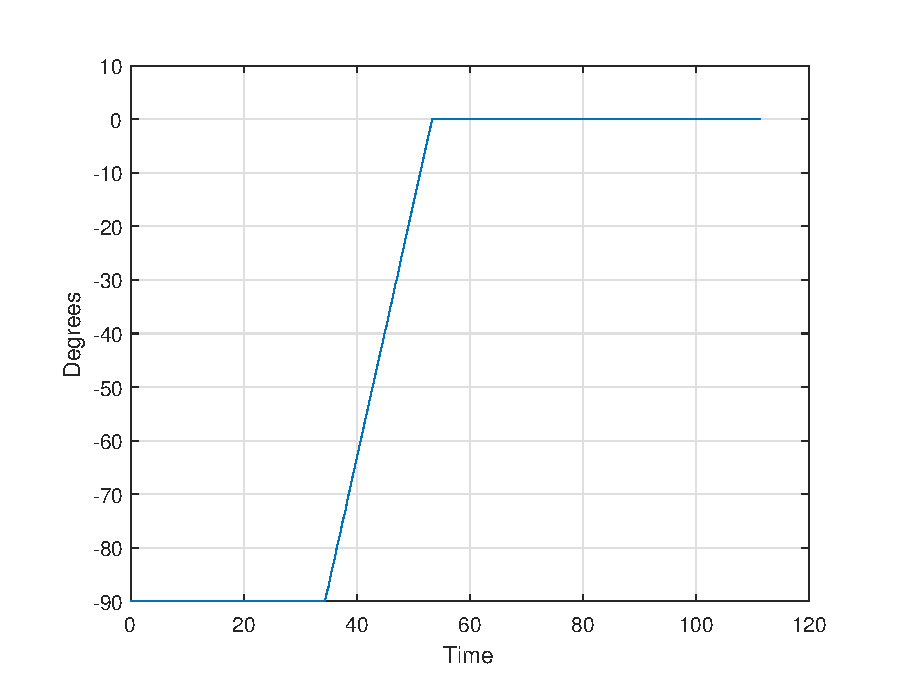
\includegraphics[width=\textwidth]{task_9_500_deg_initial_000_Goal_2090.eps}
        \caption{Initial position: (0,0) 0 degrees}
        \label{fig:deg0002090}
    \end{subfigure}
   
   
    \begin{subfigure}[b]{6cm}
        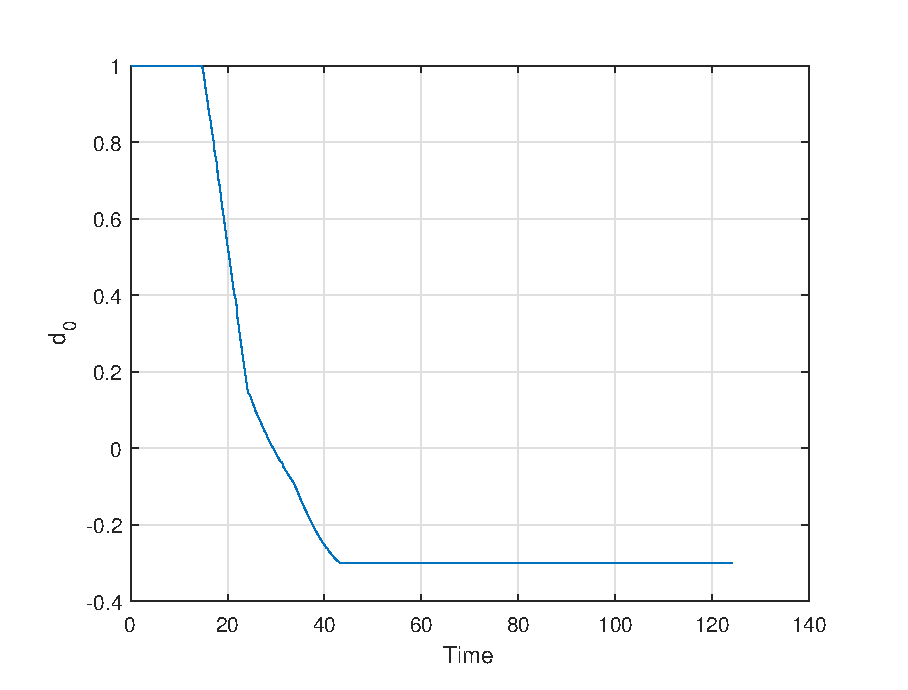
\includegraphics[width=\textwidth]{task_9_500_d0_initial_11180_Goal_2090.eps}
        \caption{Initial position: (1,1) 180 degrees}
        \label{fig:d0111802090}
    \end{subfigure}
     \begin{subfigure}[b]{6cm}
        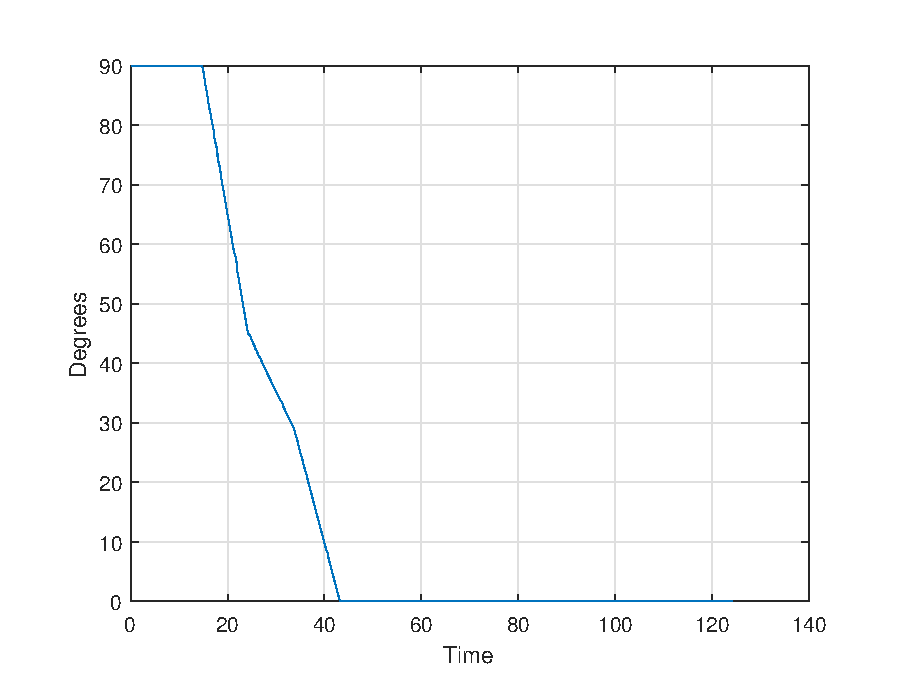
\includegraphics[width=\textwidth]{task_9_500_deg_initial_11180_Goal_2090.eps}
        \caption{Initial position: (1,1) 180 degrees}
        \label{fig:deg111802090}
    \end{subfigure}
    \caption{Goal: (2,0) 90 degrees}\label{fig:2090}
\end{figure}



\begin{figure}[H]
    \centering
    \begin{subfigure}[b]{6cm}
        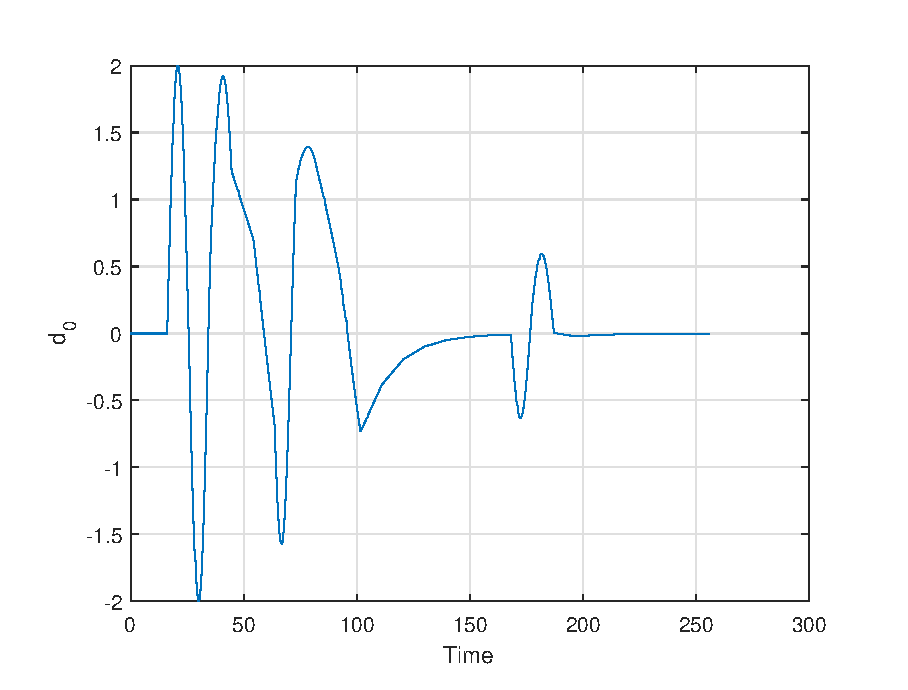
\includegraphics[width=\textwidth]{task_9_500_d0_initial_000_Goal_02180.eps}
        \caption{Initial position: (0,0) 0 degrees}
        \label{fig:d0009002180}
    \end{subfigure}
    \begin{subfigure}[b]{6cm}
        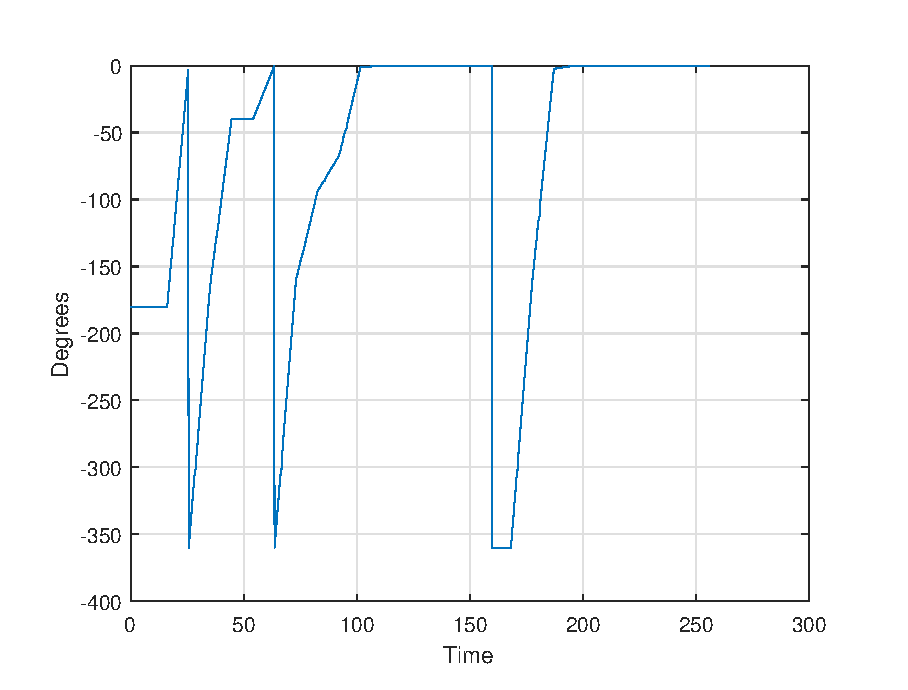
\includegraphics[width=\textwidth]{task_9_500_deg_initial_000_Goal_02180.eps}
        \caption{Initial position: (0,0) 0 degrees}
        \label{fig:deg009002180}
    \end{subfigure}
   
   
    \begin{subfigure}[b]{6cm}
        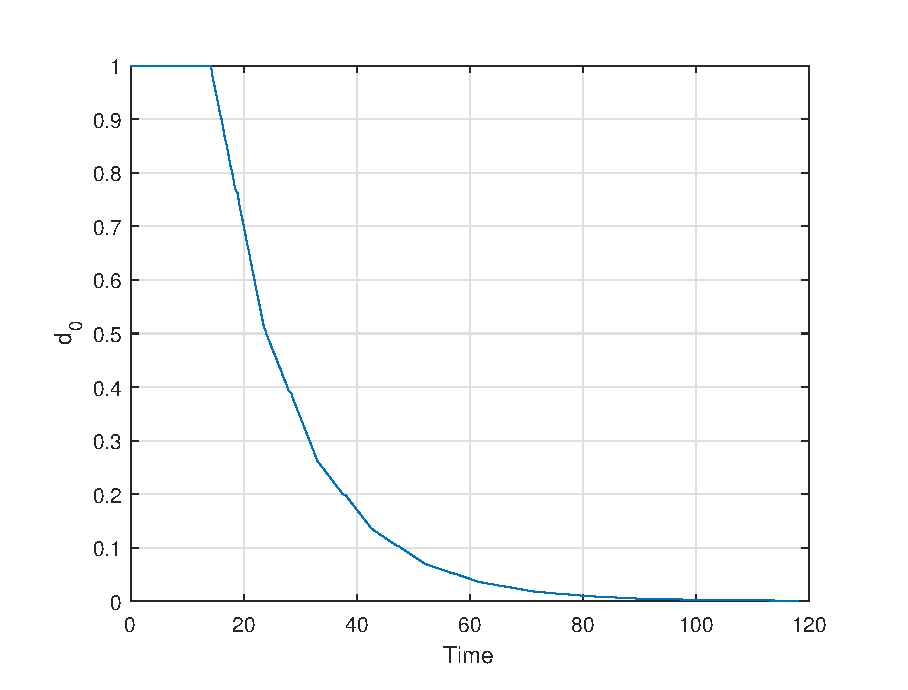
\includegraphics[width=\textwidth]{task_9_500_d0_initial_11180_Goal_02180.eps}
        \caption{Initial position: (1,1) 180 degrees}
        \label{fig:d01118002180}
    \end{subfigure}
     \begin{subfigure}[b]{6cm}
        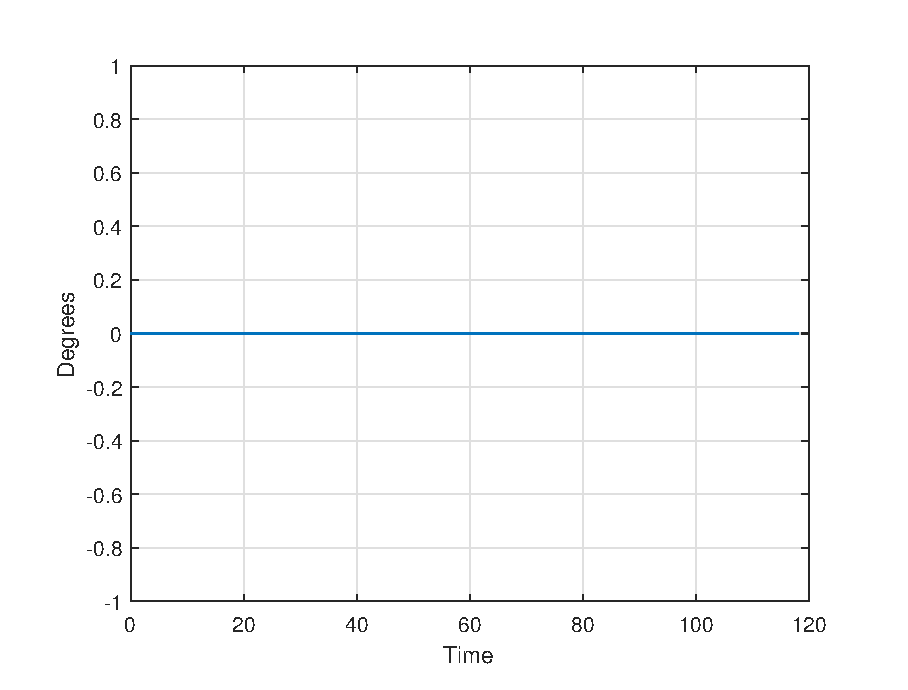
\includegraphics[width=\textwidth]{task_9_500_deg_initial_11180_Goal_02180.eps}
        \caption{Initial position: (1,1) 180 degrees}
        \label{fig:deg1118002180}
    \end{subfigure}
    \caption{Shows $d_0$ and $\theta-\theta^R$. Goal: (0,2) 180 degrees}
\end{figure}

\begin{figure}[H]
    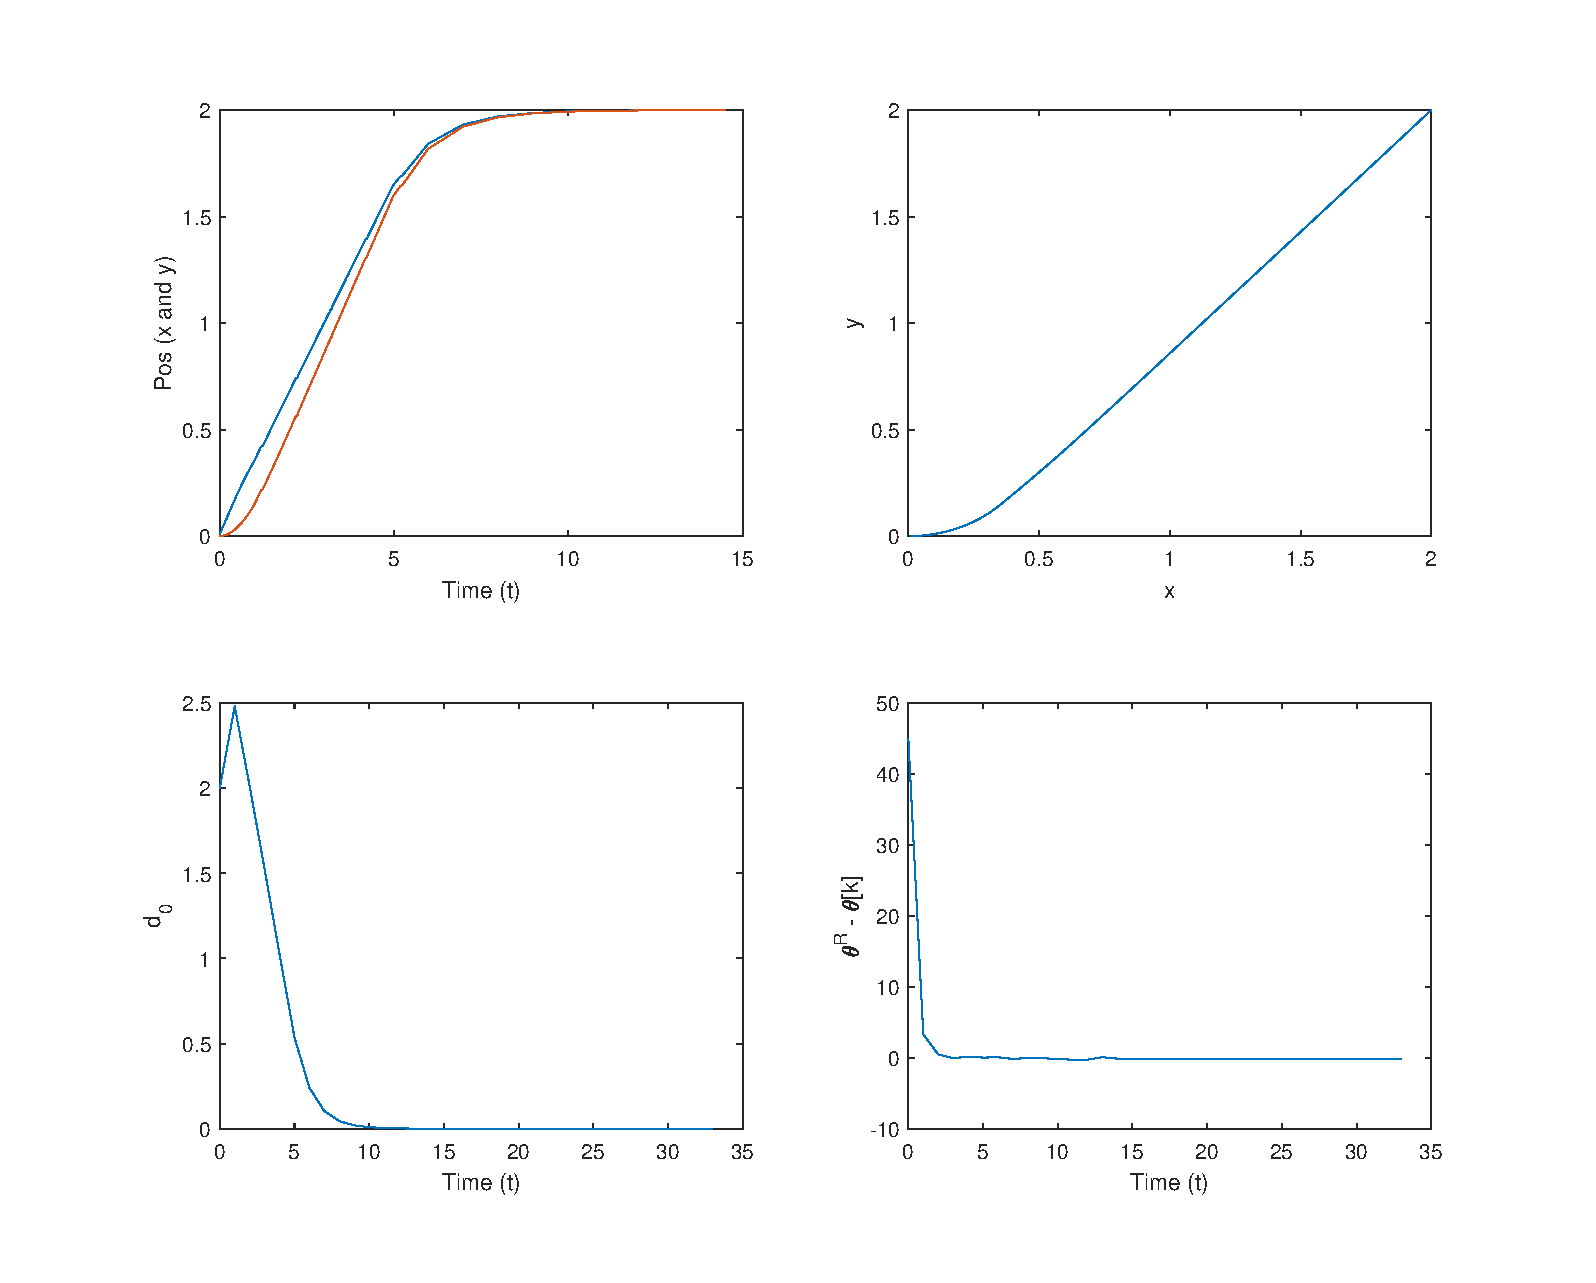
\includegraphics[width=\textwidth]{figs/perf-d0-theta.eps}
    \caption{Simulation of the combined $\Delta \theta$ and the $d_0$  controller going from $(0, 0)$ to $(2, 2)$ with $K_\omega= \frac{180}{R \pi}$ and $K_\psi= \frac{L}{R}$  }\label{fig:02180}
\end{figure}

In the first situations, the controller works fairly good. It can approach the target position first. Then it rotates toward the reference direction as it moving towards the target position simultaneously. The robot finishes the leftover rotation when it reach the target position. This is completely different from the situation when the reference direction differs greatly from the direction towards the target position. 

From the plots, some very oscillating behaviours can be observed when the desired direction and movement direction differs greatly. In these situations, the robot basically stops several times and rotates toward the desired direction and rotate back during the movement toward the desired location. This is undesired since it takes much time and create instability but does not bring any benefit. So it is not a good idea to enable both of these controller simultaneously. 

\section*{Task 10}

This proof is very similar to the one in task 7. We start with time shifting the definition of $d_p$ one step forward to get $d_0[k+1] =  v_g \cdot \Delta_g[k+1].$ Since the angle $\theta_g$ is constant $v_g$ is not a function of $k$ here.  

Just as in task 7, naming the position $p[k]$, we can express $\Delta_g[k+1]$ as
\begin{equation*}
\Delta_g[k+1] = \Delta_g[k] + p[k] - p[k+1].
\end{equation*}

The position in the next time step is given by $p[k+1] = p[k] + R\frac{\pi}{180}v[k] v_g.$ Putting the equation for the controller into the equation for the position results in $p[k+1] = p[k] + K_\omega R\frac{\pi}{180}d_g[k] v_g.$
Inserting this expression into the equation for $\Delta_g[k+1]$ we get 
\begin{equation*}
\Delta_g[k+1] = \Delta_g[k] - K_\omega R\frac{\pi}{180}d_g[k] v_g. 
\end{equation*}

Inserting this into the definition of $d_g$ gives, $d_g [k+1] = (\Delta_g[k] - R\frac{\pi}{180}d_g[k] v_c)\cdot v_c.$ Since $\Delta_g[k] \cdot v_c = \d_g[k]$ and $v_g\cdot v_g = 1$ we finally get
\begin{equation*}
d_g [k+1] = (1-K_\omega \frac{\pi}{180})d_g[k].
\end{equation*}

The eigenvalue of this system is given by $1-K_\omega \frac{\pi}{180}.$ If $K_\omega > 2\frac{180}{R \pi}$ the system will become unstable. $K_\omega = \frac{180}{R \pi} \approx 572$ gives a dead beat controller.

\section*{Task 11}

\begin{figure}[H]
    \centering
    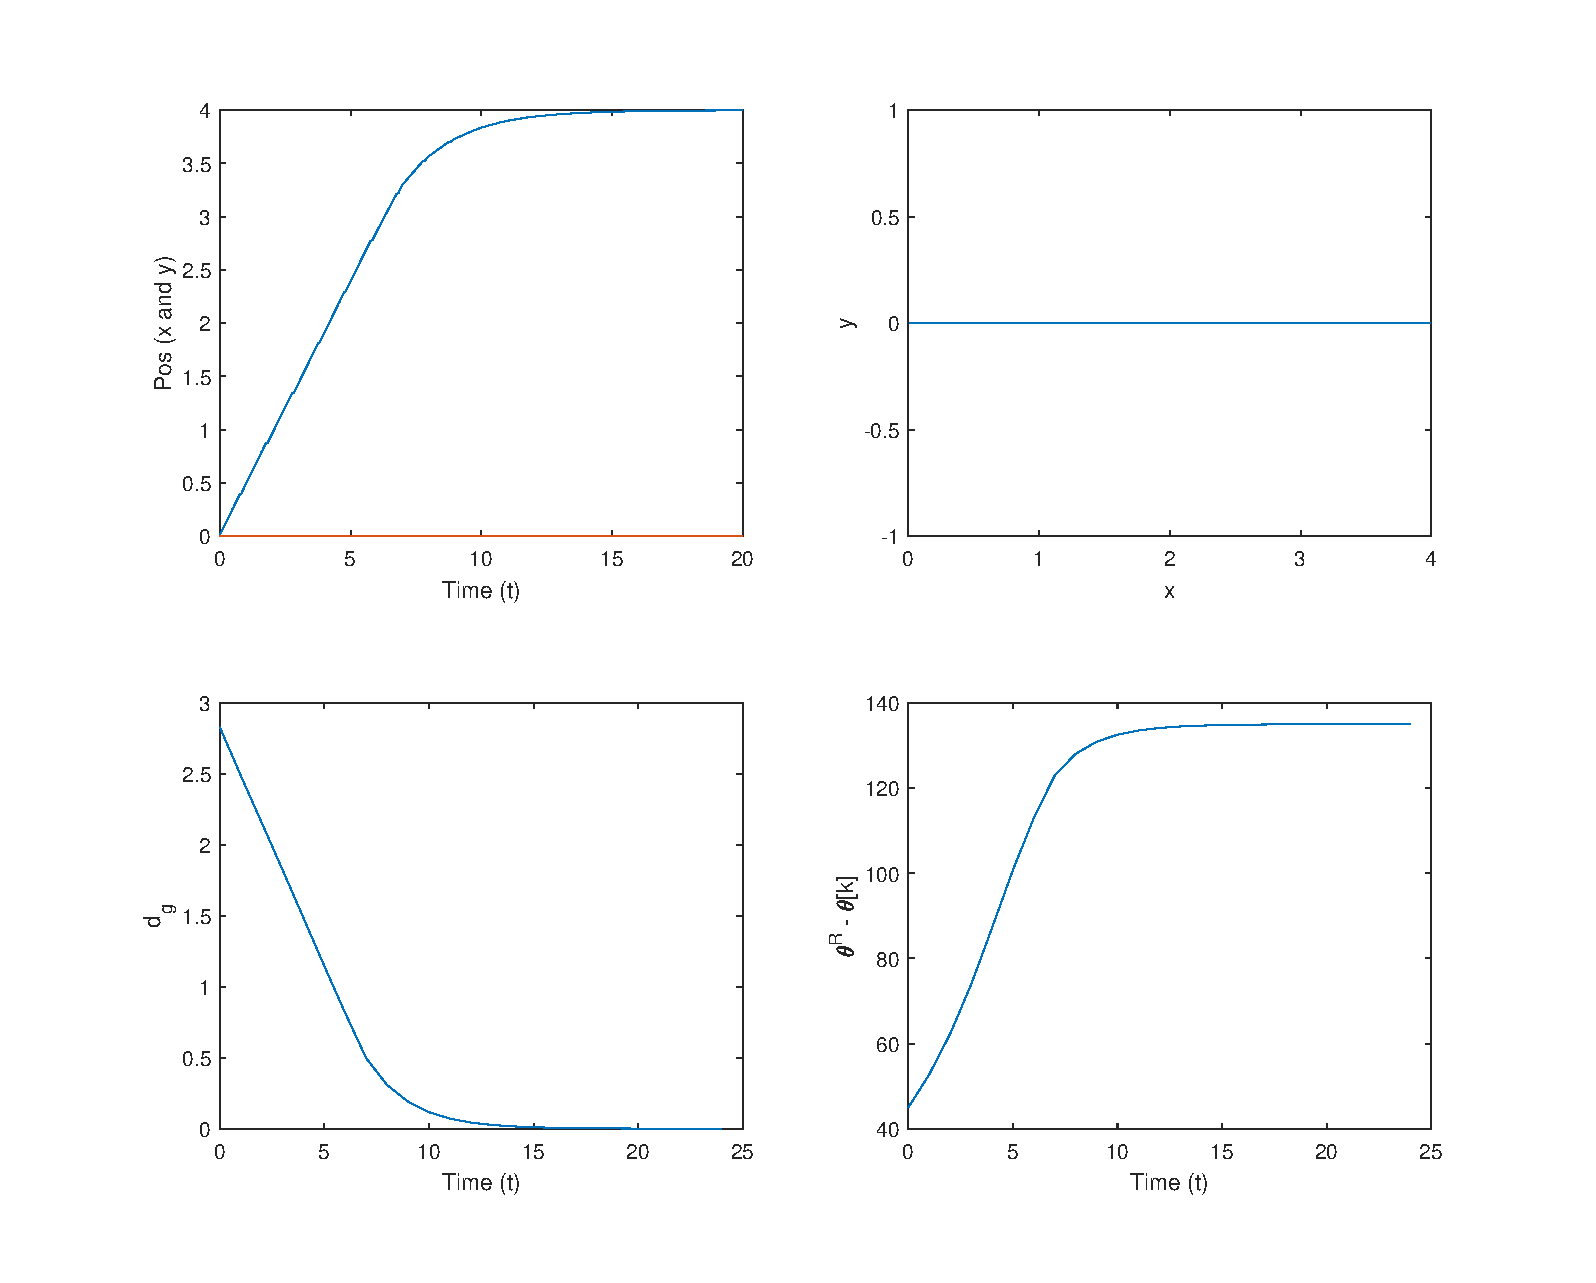
\includegraphics[width=\textwidth]{figs/perf-dg.eps}
    \caption{Simulation of the $d_g$  controller going from $(0, 0)$ to $(2, 2)$ with $K_\omega= \frac{180}{R \pi}.$}\label{fig:perf-dg}
\end{figure}

The controller drives the robot to a position orthogonal to the goal position on the line between $(x_0, y_0)$ and $(x_g, y_g)$. Since $K_\omega$ is set to give a dead beat controller the robot should get close to to the goal position if it starts in the direction of the goal. Otherwise it will not reach the goal position.

\section*{Task 12}

According to the definition, $d_p$ can be expressed in the following way.
\begin{equation}
\begin{aligned}
    d_p = & 
    \begin{bmatrix}
    \sin{\theta_g} & -\cos{\theta_g} \\
    \end{bmatrix} \cdot  
    \begin{bmatrix}
    x(k) - x_0 + p \cdot \cos{\theta[k]} \\
    y(k) - y_0 + p \cdot \sin{\theta[k]} 
    \end{bmatrix} \\
    = & (\sin{\theta_g}(x(k) - x_0) - \cos{\theta_g}(y(k) - y_0)) + p[\sin{\theta_g}\cos{\theta[k]} - \cos{\theta_g}\sin{\theta[k]}] \\
    = & (\sin{\theta_g}(x(k) - x_0) - \cos{\theta_g}(y(k) - y_0)) + p \sin{(\theta_g-\theta[k])}
\end{aligned}
\end{equation}

If the robot is on the line between $(x_0, y_0)$ and $(x_g, y_g)$, the position of the robot is orthogonal to $v_{g,\perp},$, so $(\sin{\theta_g}(x(k) - x_0) - \cos{\theta_g}(y(k) - y_0)) = 0.$ Also, if $\theta_g \approx \theta[k],$ then $p \sin{(\theta_g-\theta[k])} \approx p (\theta_g-\theta[k])$ (from the Taylor expansion of $\sin$). The scalar product can then be expressed as 
\[
d_p = p(\theta_g - \theta[k]).
\]

Inserting this expression for $d_p$ into the formula for the controller yields $\omega[k] \approx K_\psi p \frac{\pi}{180} (\theta_g - \theta[k]).$ Time shifting the expression for the approximation of $d_g$ gives $d_g[k+1] = p(\theta_g - \theta[k]).$ The angle $\theta[k+1] = \theta[k] + \frac{R}{L} \omega[k] \approx \theta[k] + \frac{R}{L}K_\psi p  \frac{\pi}{180}(\theta_g - \theta[k]).$Inserting this back into the equation for $d_p[k+1]$ results in
\[
    d_p[k+1] \approx p ( (1-K_\psi p  \frac{\pi}{180}\frac{R}{L}) \theta_g - (1 - K_\psi p  \frac{\pi}{180} \frac{R}{L}) \theta[k])
\]
which is zero when $K_\psi =  \frac{180}{\pi}\frac{L}{Rp}.$

%When $\theta_g \approx \theta$, we have:
%\begin{equation}
%    \begin{aligned}
%    \frac{\sin{\theta_g}}{\cos{\theta_g}} = \tan{\theta_g} \approx \tan{\theta[k]} = \frac{y(k)-y_0}{x(k)-x_0} \\ \Rightarrow \sin{\theta_g}(x(k) - x_0) - \cos{\theta_g}(y(k) - y_0) \approx 0 \\
%    p \sin{\theta_g-\theta[k]} \approx p (\theta_g - \theta[k])
%    \end{aligned}
%\end{equation}
%Then the following approximating formula can be deduced. 
%\begin{equation}
%    \omega[k] = K_\psi p (\theta_g - \theta[k])
%\end{equation}
%which is similar to the task 5 thus a similar result can be applied. 

\section*{Task 13}

$p$ is the importance of how much the angle matters compared to how much the robots distance from the line matters. A large value of $p$ will give more weight to the angle but be more lenient of transnational errors, while a small $p$ will make the robot turn more to stay on the line, but less to keep the direction of the line. $p$ is a additional proportional controller that applies on the angular velocity so it scales $K_\omega$. This can lead to instability or larger oscillation in the $\theta$ coordinate. In the stable situation with a large $p$, the robot will still be able to follow a line. But it will oscillate around the line as it following the line. So it will be harder to following the line perfectly. 


\section*{Task 14}

\begin{figure}[H]
    \centering
    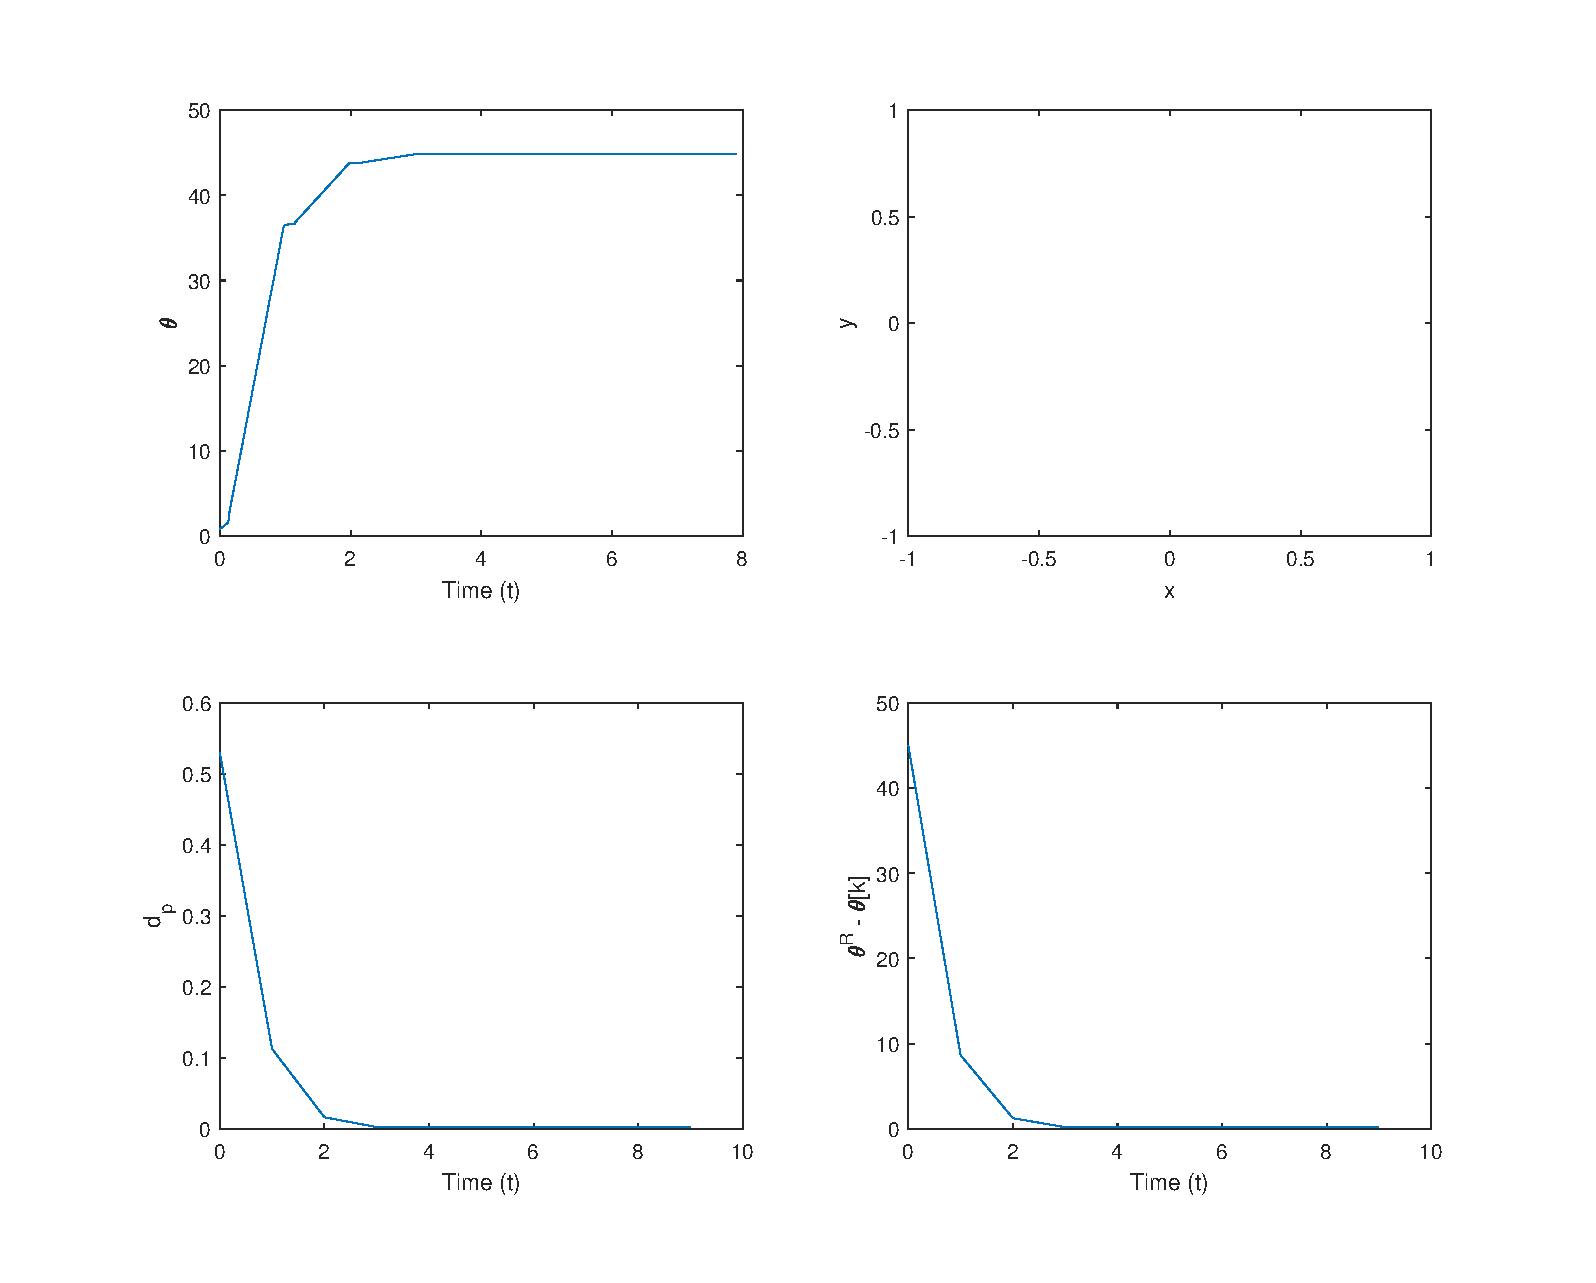
\includegraphics[width=\textwidth]{figs/perf-dp.eps}
    \caption{Simulation of the $d_p$ controller going from $(0, 0)$ to $(2, 2)$ with $K_\psi = \frac{180}{\pi} \frac{L}{Rp}$ and $p = 0.75$}\label{fig:perf-dg}
\end{figure}

The error $d_p[k]$ will go to 0 since $K_\phi$ is set to give  deadbeat controller.

\section*{Task 15}

\begin{figure}[H]
    \centering
    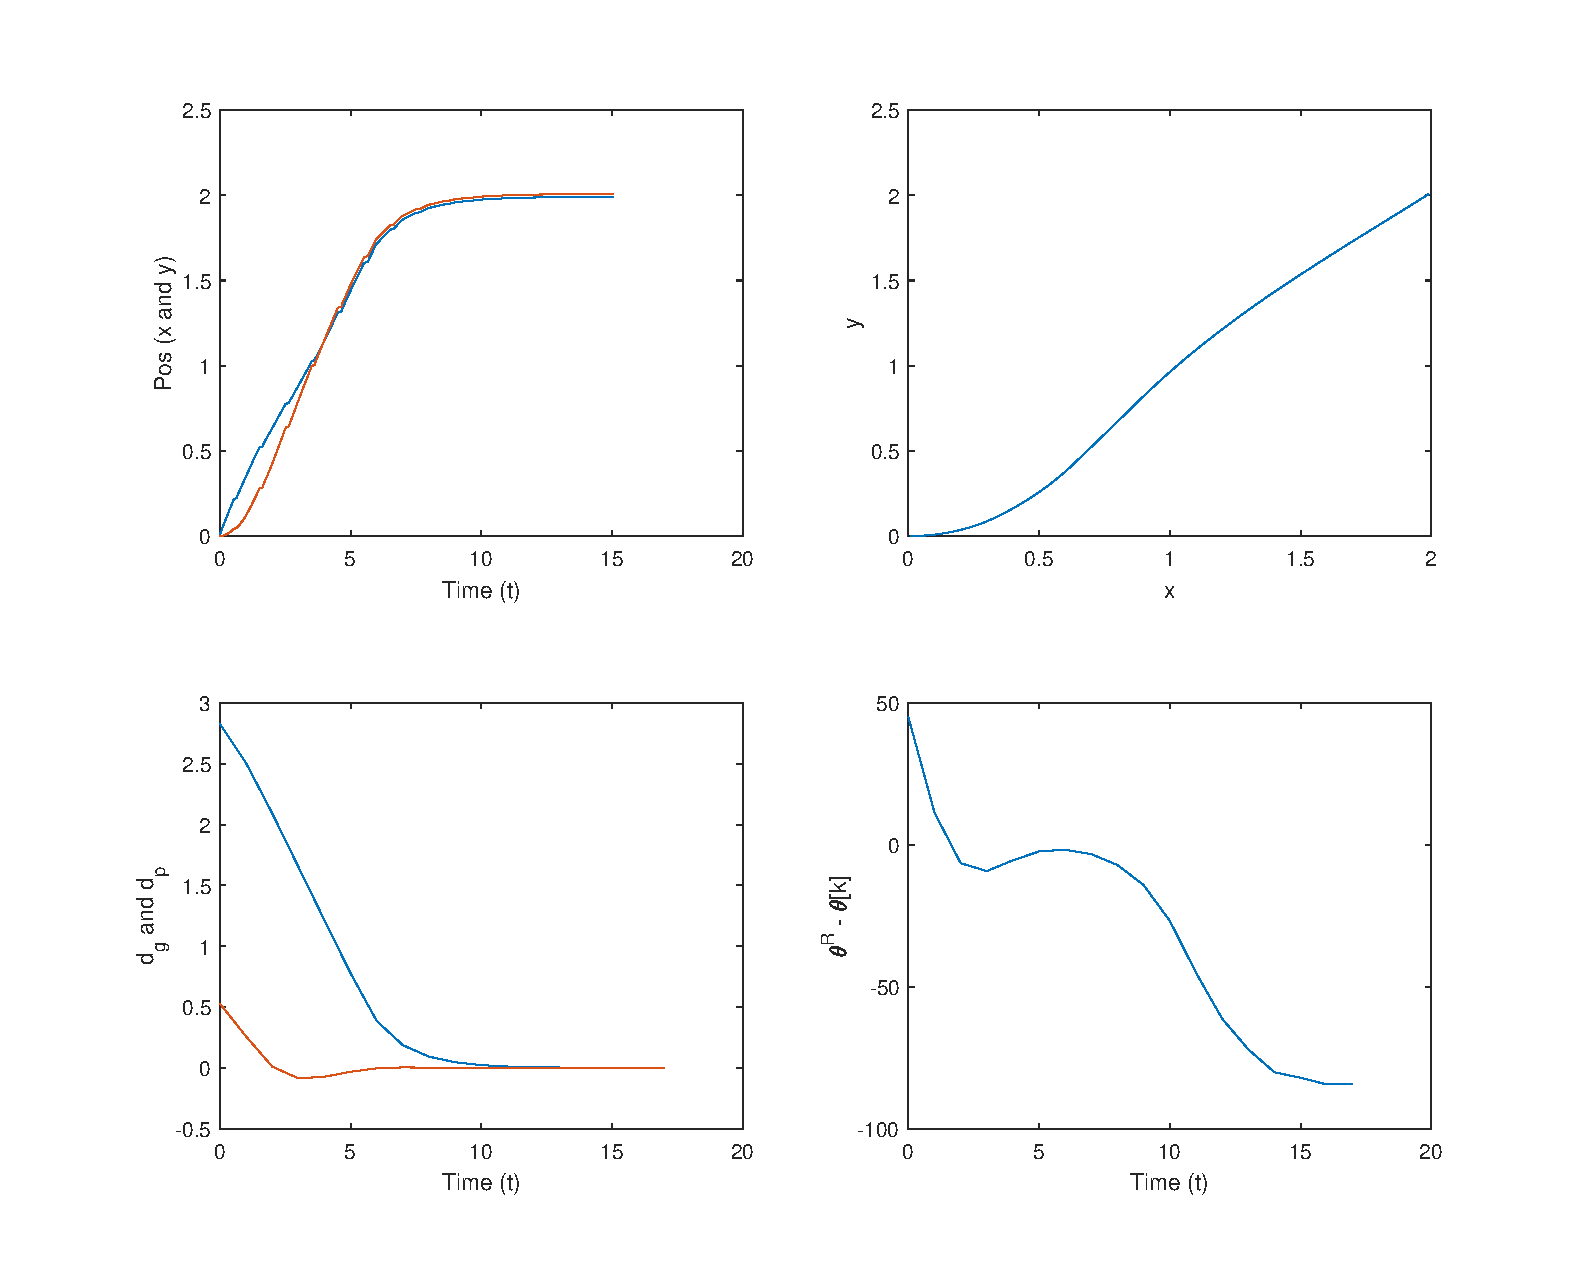
\includegraphics[width=\textwidth]{figs/perf-follow.eps}
    \caption{Simulation of the combined $d_g$ and $d_p$ controller going from $(0, 0)$ to $(2, 2)$ with $K_\omega = \frac{180}{R\pi}$, $K_\psi = \frac{180}{\pi} \frac{L}{Rp}$ and $p = 0.75$}\label{fig:perf-dg}
\end{figure}

As can be seen in \ref{fig:perf-dg}, the $d_g$ error evolve in an almost identical way to when the controller is used separately. However the $d_p$ error get a small overshoot compared to the separate case. This is likely from the virtual point getting pushed through the line by the velocity controller.

\section*{Task 16}

The hybrid controller is modeled as a three state system. Where $q_1$ is when the robot is at the initial position and rotates to the direction of the goal position. It enters the next state $q_2$ when the direction of the robot is sufficiently near the desired direction. In state $q_2$ the robot drives towards the goal destination. When the robot is sufficiently close the goal position the controller enters state 3, $q_3$, which is the final state where the robot has completed its mission. 

\begin{align*}
H &= (Q,X,Init,f,D,E,G,R)\\
&\textrm{Where: }\\
Q &= (q_1,q_2,q_3)\\
X &= (x,y,\theta)\\
Init &= (q_1,x_0,y_0,\theta_0)\\
f(q_1, x, y, \theta) &= \left[0,\ 0,\ K_\psi(\theta-\theta^R))\right]^T \\
f(q_2, x, y, \theta) &= \left[  K_\omega d_g cos(\theta),\ K_\omega d_g sin(\theta),\ K_\psi \frac{180}{\pi p} \right]^T \\
f(q_3, x, y, \theta) &= \left[0, 0, 0\right]^T \\
%D(q_1) &= [x,y,\theta]\in [\textrm{Constant } A \in \mathbb{R}, \textrm{Constant } B \in \mathbb{R},0\leq\theta\leq360^o    ]\\
D(q_1) &= [x,y,\theta]\in [\textrm{Constant } A \in \mathbb{R},\ \textrm{Constant } B \in \mathbb{R}, \ -180^o\leq\theta\leq 180^o    ]\\
%D(q_2) &= [x,y,\theta]\in [\mathbb{R}, \mathbb{R}, \textrm{Constant } \theta | \ -180^o\leq\theta\leq 180^o  ]\\
D(q_2) &= [x,y,\theta]\in [\mathbb{R},\ \mathbb{R},\ -180^o\leq\theta\leq 180^o   ]\\
D(q_3) &= [\textrm{Constant } A \in \mathbb{R},\ \textrm{Constant } B \in \mathbb{R},\ \mathbb{R}, \textrm{Constant } \theta | 0\leq\theta\leq360^o   ]    ]\\
E&=\{(q_1, q_2), (q_2, q_3), (q_3, q_1) \}\\
G(q_1, q_2) &= \{|\theta-\theta^R|<10^o \}\\
G(q_2, q_3) &= \{|x_0-x_g|<3cm,|y_0-y_g|<3cm\}\\
G(q_3, q_1) &= \textrm{When a new goal point is inputted} \\
R(e)&= x \leftarrow x,\ y \leftarrow y,\ \theta \leftarrow \theta \ \forall e \in E
\end{align*}  

\section*{Task 17}

\begin{figure}[H]
    \centering
    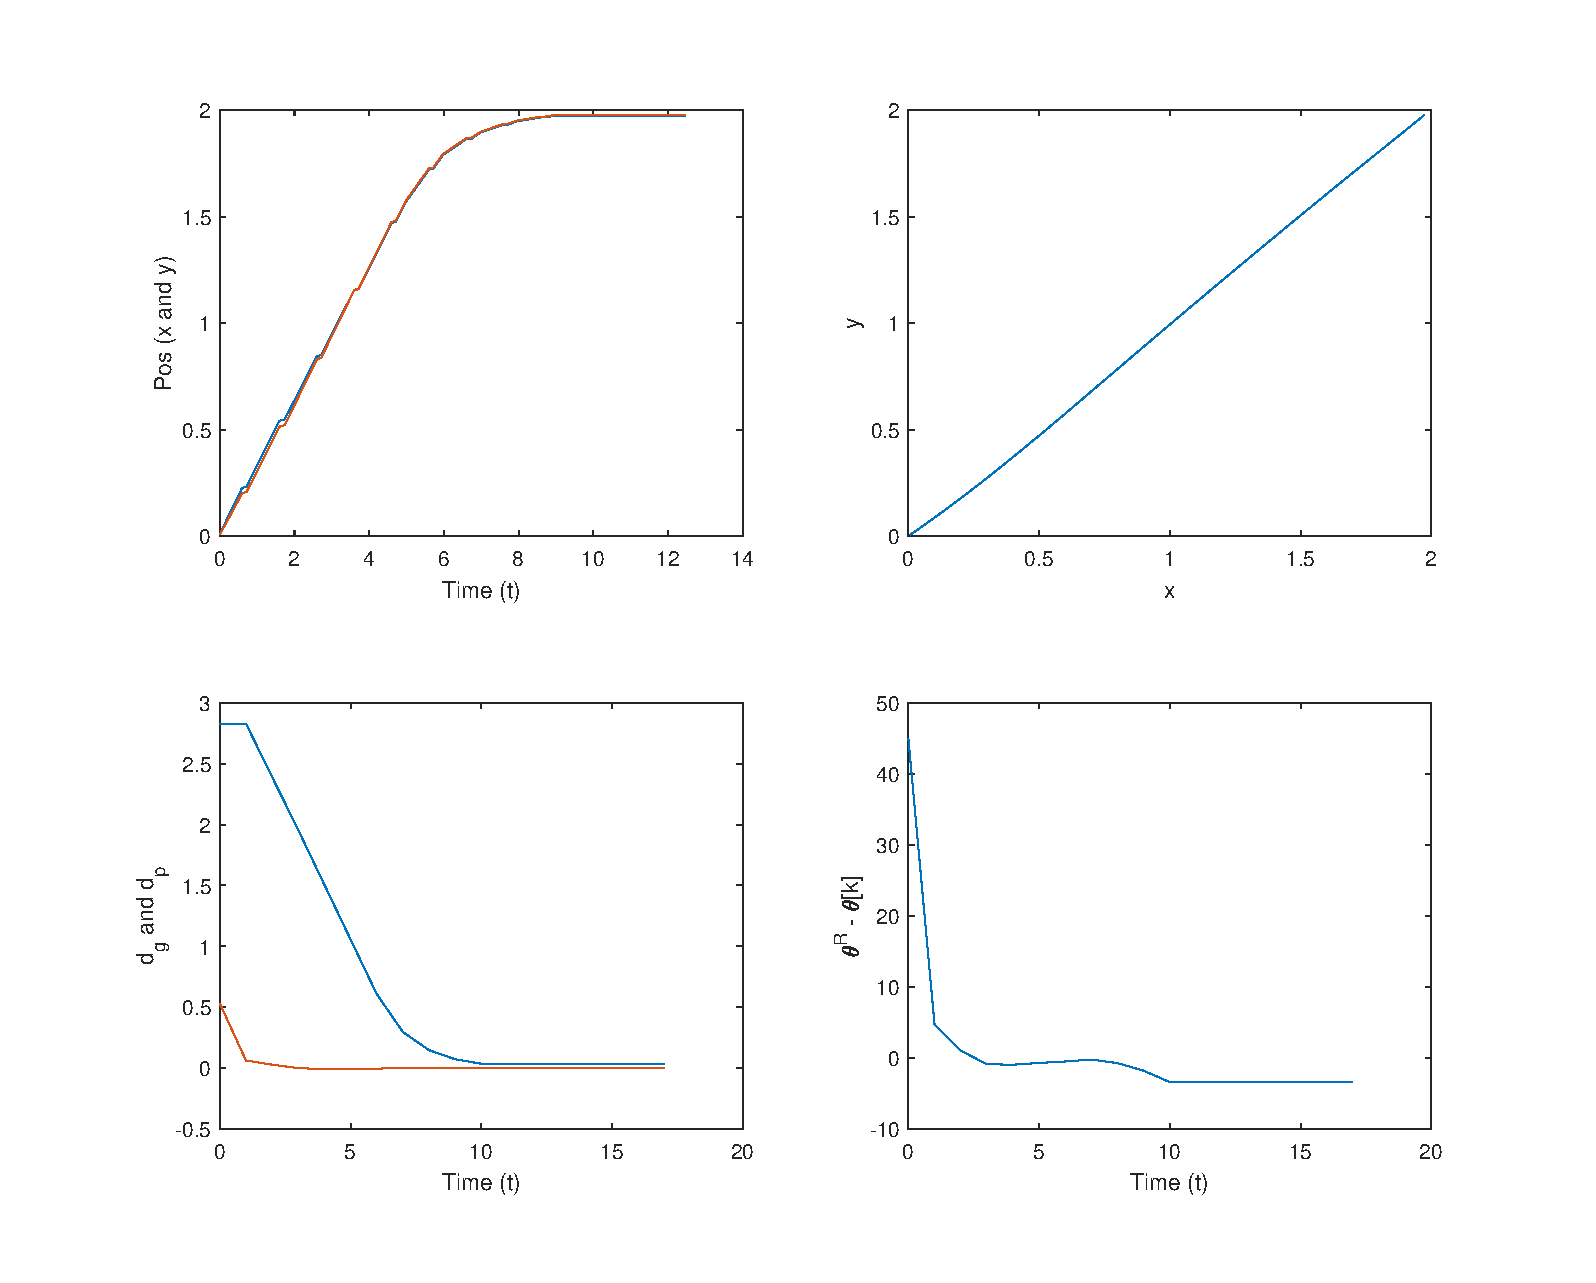
\includegraphics[width=\textwidth]{figs/perf-hybrid.eps}
    \caption{Simulation of the hybrid controller going from $(0, 0)$ to $(2, 2)$ with $K_\omega = \frac{180}{R\pi}$, and $p = 0.75.$ The directional controller has $K_\psi = \frac{L}{R}$ and the got to goal controller uses $K_\psi = \frac{180}{\pi} \frac{L}{Rp}$} \label{fig:perf-hybrid}
\end{figure}

\begin{figure}[H]
    \centering
    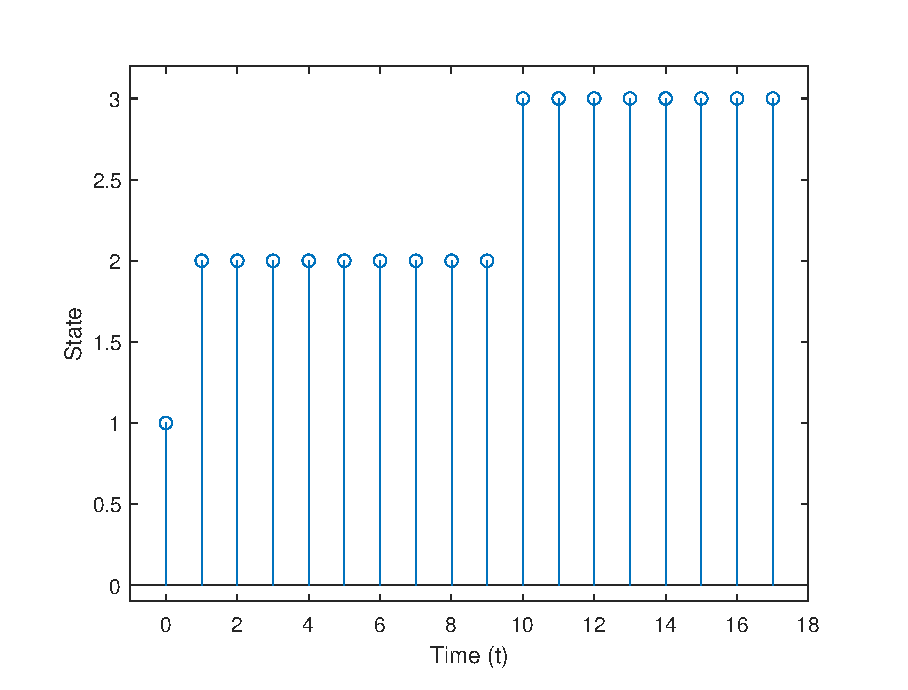
\includegraphics[width=\textwidth]{figs/state.eps}
    \caption{The sequence of discrete states of the hybrid controller going from $(0, 0)$ to $(2, 2)$ with a starting angle of 0. } \label{fig:states}
\end{figure}

The discrete state would be expected to first go into $q_1$ for a short while when the robot turns towards the direction of the goal. Then it should go into state $q_2$ for a while when driving towards the goal, and finally it should end up in state 3 when it has reached the goal. This is the exact behavior that is shown in figure \ref{fig:states}.

\section*{Task 18}

\begin{figure}[H]
    \centering
    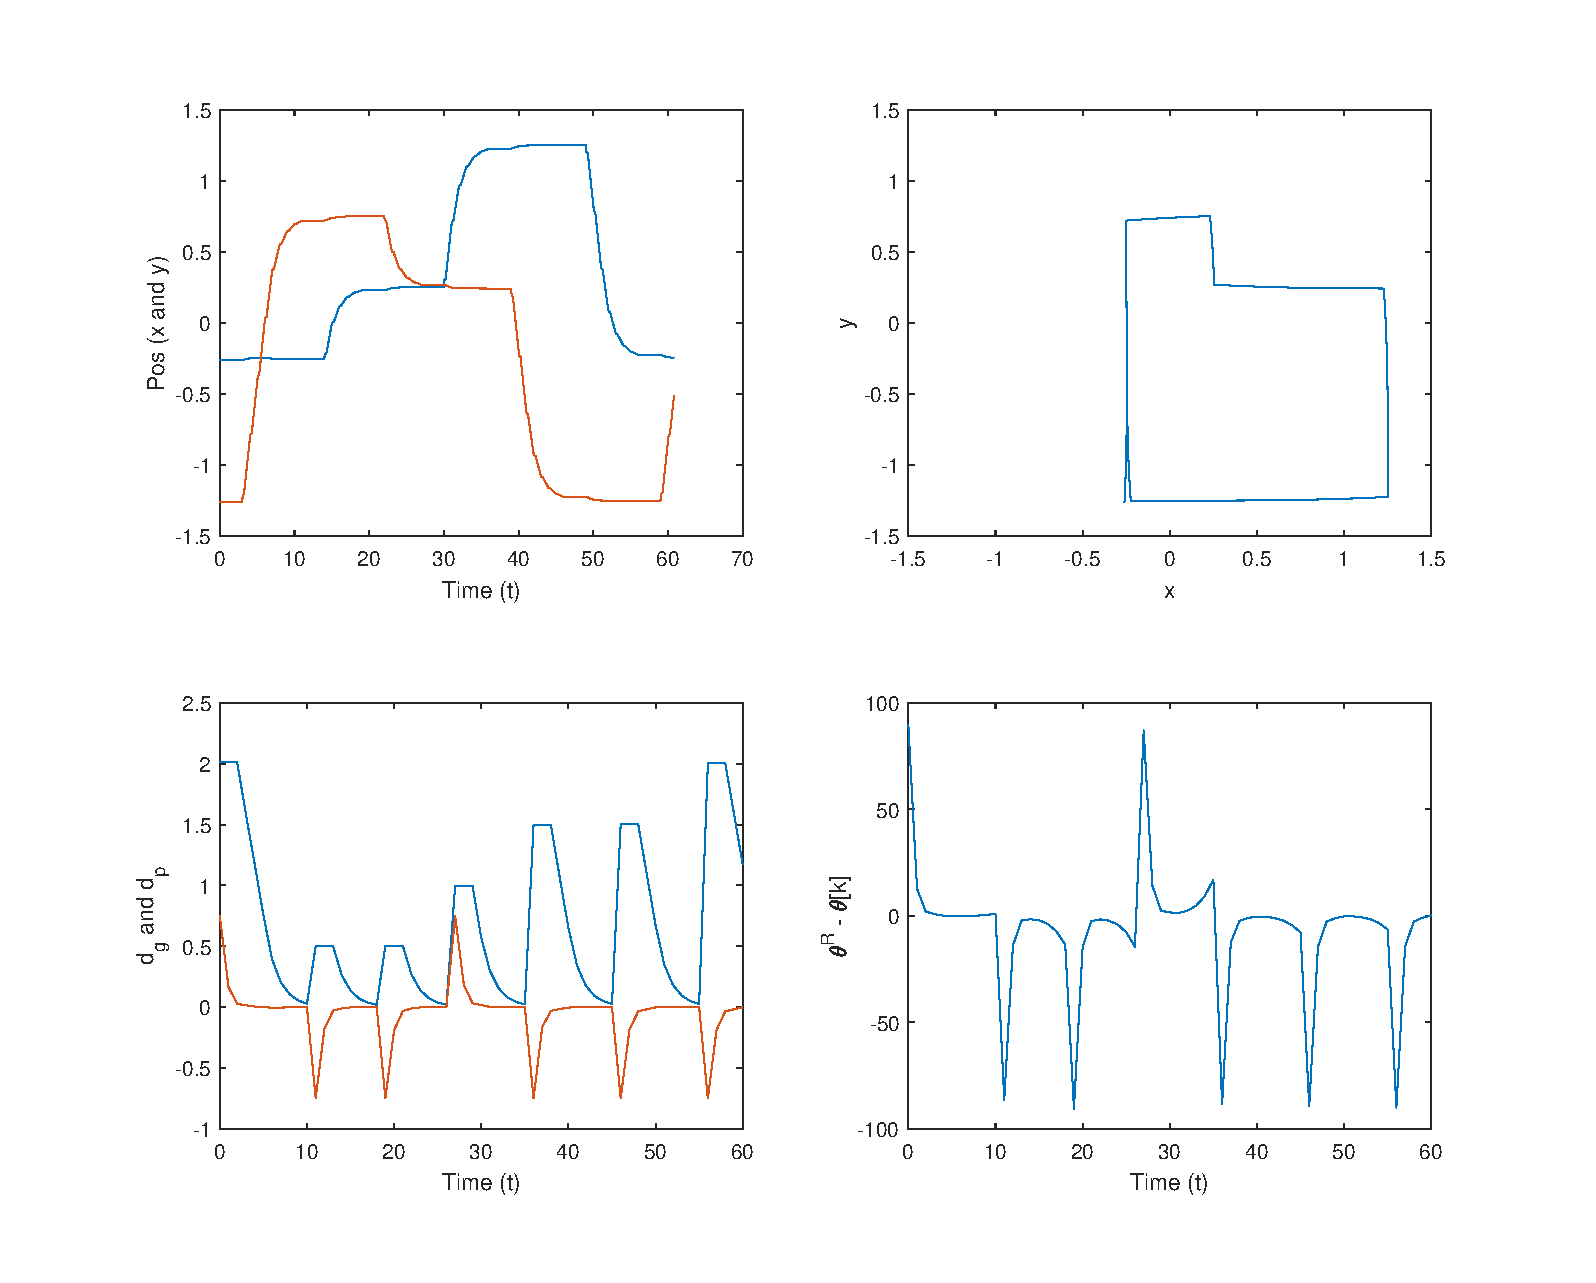
\includegraphics[width=\textwidth]{figs/perf-fullrun.eps}
    \caption{Simulation of a full run with the hybrid controller going from $(0, 0)$ to $(2, 2)$ with $K_\omega = \frac{180}{R\pi}$, and $p = 0.75.$ The directional controller has $K_\psi = \frac{L}{R}$ and the got to goal controller uses $K_\psi = \frac{180}{\pi} \frac{L}{Rp}$} \label{fig:perf-full}
\end{figure}

\begin{figure}[H]
    \centering
    \includegraphics[width=\textwidth]{figs/states-full.eps}
    \caption{The sequence of discrete states of the hybrid controller for a full run. } \label{fig:states-full}
\end{figure}

As can be seen in figure \ref{fig:perf-full}, the robot performed reasonably well. There are some concerns that the behavior is a bit uncontrolled, which might have caused it to occasionally cross into a forbidden state. A plot displaying the robots full radius from the path combined by a grid showing the states would have been interesting.



\section*{Task 19}

There are two properties of the continuous controller that can affect the safety of the property of transitions. The first is how well the robot following the line and the second is how well it stays close to the goal point. 

If the robot cannot stay in the line then the distance between the robot and the line can be large. This might leads to that the robot leave the transition regions. The problem is mainly caused by a oscillating angular controller. This can be avoid by reduce the error marginal in the direction coordinate so the robot shall move toward the target mostly. 

The second problem comes up when the speed controller is oscillating or unstable. When this occurs to stay close to the target point will be difficult. The robot might move too far away from the target and thus leave the transition regions. This can also occur in the beginning of line-tracking as well. So the solution to this problem is to minimize the oscillation of the speed controller. 



%%%%%%%%%%%%%%%%%%%%%%%%%%%%%%%%%%%%%%%%%%%%%%%%%%%%%%%%%%%%%%%%%%%%%%%%%%%%%%%%%%%
% The bibliography
%%%%%%%%%%%%%%%%%%%%%%%%%%%%%%%%%%%%%%%%%%%%%%%%%%%%%%%%%%%%%%%%%%%%%%%%%%%%%%%%%%%
%\bibliography{Bibliography_template} %Read the bibliography from a separate file

\begin{thebibliography}{99}
\bibitem[Khalil(2002)]{Khalil:2002:Nonlinear-systems:vh}
Hassan~K Khalil.
\newblock \emph{Nonlinear systems}.
\newblock Prentice Hall, Upper Saddle river, 3. edition, 2002.
\newblock ISBN 0-13-067389-7.

\bibitem[Oetiker et~al.(2008)Oetiker, Partl, Hyna, and
  Schlegl]{Oetiker:2008:TheNotSoShortIntroductiontoLaTeXe}
Tobias Oetiker, Hubert Partl, Irene Hyna, and Elisabeth Schlegl.
\newblock \emph{The Not So Short Introduction to \LaTeXe}.
\newblock Oetiker, OETIKER+PARTNER AG, Aarweg 15, 4600 Olten, Switzerland,
  2008.
\newblock http://www.ctan.org/info/lshort/.

\bibitem[Sastry(1999)]{Sastry:1999:Nonlinear-systems:-analysis-stability-and-c%
ontrol:xr}
Shankar Sastry.
\newblock \emph{Nonlinear systems: analysis, stability, and control},
  volume~10.
\newblock Springer, New York, N.Y., 1999.
\newblock ISBN 0-387-98513-1.
\end{thebibliography}


\end{document}      % End of the document
